\documentclass[12pt,a4paper]{report}
\usepackage[utf8]{inputenc}
\usepackage[french]{babel}
\usepackage[T1]{fontenc}
\usepackage{times}
\usepackage[left=2cm,right=2cm,top=2cm,bottom=2cm]{geometry}
\usepackage{fancybox}
\usepackage{color}
\usepackage{setspace}
\usepackage{graphicx}
\usepackage{amsmath, amsfonts, amssymb}
\usepackage[pdfauthor={{YAKHOUB MAHAMAT HAMDO}},
            pdftitle={{CyberSentinel-LLM}},
            pdfstartview=Fit,
            pdfpagelayout=SinglePage,
            pdfnewwindow=true,
            bookmarksnumbered=true,
            breaklinks,
            colorlinks,
            linkcolor=blue,
            urlcolor=black,
            citecolor=cyan,
            linktoc=all]{hyperref}
\usepackage{array}
\usepackage{xcolor}
\usepackage{float}
\usepackage{enumitem, pifont}
\usepackage{amssymb}
\usepackage{booktabs}
\usepackage{longtable}
\usepackage{caption}
\usepackage{subcaption}
\definecolor{darkblue}{RGB}{4, 89, 187}
\definecolor{lightblue}{RGB}{220, 235, 255}
\definecolor{gold}{RGB}{212, 175, 55}
\usepackage{tcolorbox}
\tcbuselibrary{skins}
\usepackage{fancyhdr}
\usepackage{emptypage}
\usepackage{tikz}
\usetikzlibrary{calc}
\usepackage{titlesec}
\usepackage{titletoc}
\usepackage[Glenn]{fncychap}
\usepackage{soul}
\usepackage[normalem]{ulem}
\renewcommand{\arraystretch}{1.3}

\begin{document}
\pagenumbering{Roman}
\thispagestyle{empty}

%% ============================================================
%% PAGE DE GARDE
%% ============================================================
\begin{titlepage}

\tikz[overlay, remember picture]{
  \draw [darkblue, line width=4pt]
    ([xshift=1.0cm, yshift=-1.0cm]current page.north west)
    rectangle
    ([xshift=-1.0cm, yshift=1.0cm]current page.south east);
  \draw [gold, line width=1.2pt]
    ([xshift=1.35cm, yshift=-1.35cm]current page.north west)
    rectangle
    ([xshift=-1.35cm, yshift=1.35cm]current page.south east);
}

\vspace{0.3cm}

\begin{center}
  \hspace{2cm}
\includegraphics[width=0.60\textwidth]{images/enastic_logo2.png}
\end{center}

\vspace{0.2cm}

\begin{center}
  \begin{tcolorbox}[
    enhanced,
    colback=lightblue,
    colframe=darkblue,
    arc=6pt,
    boxrule=1.5pt,
    width=0.92\textwidth,
    halign=center
  ]
    \textbf{\large Projet de Fin d'Études}\\[4pt]
    {\normalsize En vue de l'obtention du \textbf{Diplôme de Licence en Informatique}}
  \end{tcolorbox}
\end{center}

\vspace{0.4cm}

\begin{center}
  \begin{tcolorbox}[
    enhanced,
    colback=darkblue,
    colframe=gold,
    arc=8pt,
    boxrule=2pt,
    width=\textwidth,
    halign=center
  ]
    \vspace{0.2cm}
    {\color{white}\large\textbf{\underline{THÈME}}}\\[6pt]
    {\color{white}\Large\textbf{CyberSentinel-LLM :}}\\[4pt]
    {\color{white}\large Plateforme Cognitive de Cybersécurité Conversationnelle}\\[2pt]
    {\color{white}\large pour la Détection Contextuelle et la}\\[2pt]
    {\color{white}\large Neutralisation Adaptive des Menaces Réseau}
    \vspace{0.2cm}
  \end{tcolorbox}
\end{center}

\vspace{1cm}

\begin{flushleft}
  \textbf{\underline{Présenté par} :} \hspace{81mm} \textbf{\underline{Directeur de mémoire} :}\\[6pt]
  M. YAKHOUB MAHAMAT HAMDO \hspace{40mm} Dr. MOUAZ MICKAIL\\
  \hspace{107mm} {\small\textit{Enseignant chercheur en IA}}
\end{flushleft}

\vspace{4cm}

\begin{center}
  \begin{tcolorbox}[
    enhanced,
    colback=darkblue,
    colframe=gold,
    arc=20pt,
    boxrule=1.5pt,
    width=0.6\textwidth,
    halign=center
  ]
    \textcolor{white}{\textbf{\large Année Universitaire : 2025--2026}}
  \end{tcolorbox}
\end{center}

\end{titlepage}

%% ============================================================
%% AVANT-PROPOS
%% ============================================================
\chapter*{Avant-propos}
\addcontentsline{toc}{chapter}{Avant-propos}
\begin{onehalfspace}
L'École Nationale Supérieure des Technologies de l'Information et de la
Communication (ENASTIC) est un établissement public d'enseignement, de
recherche, d'innovation et de formation supérieure dans les domaines des
communications électroniques. Elle est créée par l'Ordonnance
\textbf{N°005/PR/2015} du 02 mars 2015, dotée de la personnalité juridique
et de l'autonomie financière.\\

Placée sous la tutelle du Ministère des Postes et des Nouvelles Technologies
de l'Information et de la Communication, et du Ministère de l'Enseignement
Supérieur, de la Recherche et de l'Innovation pour l'organisation académique
et pédagogique, l'ENASTIC a pour missions de :

\begin{itemize}
  \item[\ding{43}] Assurer la formation initiale et continue des cadres dans
  les domaines des Technologies de l'Information et de la Communication ;
  \item[\ding{43}] Entreprendre la recherche appliquée d'intérêt général, en
  vue de promouvoir l'innovation pour le développement socio-économique du
  pays ;
  \item[\ding{43}] Former des jeunes à la culture scientifique afin de les
  rendre aptes à élaborer et à porter des projets structurants adossés aux TIC.
\end{itemize}

Pour compléter leurs connaissances théoriques, les étudiants doivent préparer
un Projet de Fin d'Études (PFE) afin de le présenter devant un jury de
soutenance pour parachever leur cycle de Licence.\\

C'est dans cette optique que le présent mémoire vient marquer la fin de notre
cursus en Informatique à l'ENASTIC, sur le thème :
\textbf{« CYBERSENTINEL-LLM : PLATEFORME COGNITIVE DE CYBERSÉCURITÉ
CONVERSATIONNELLE POUR LA DÉTECTION CONTEXTUELLE ET LA NEUTRALISATION
ADAPTIVE DES MENACES RÉSEAU »}, dans le cadre de l'année universitaire
2025--2026.\\

Ce travail constitue une preuve de concept pédagogique combinant détection
d'anomalies par Machine Learning, raisonnement contextuel par LLM enrichi
de MITRE ATT\&CK via RAG, et neutralisation adaptive des menaces par blocage
applicatif à validation humaine, afin d'aider les analystes SOC à interpréter,
prioriser et neutraliser les incidents de sécurité. Le travail porte sur la
conception, l'implémentation d'un prototype fonctionnel, et l'évaluation de
ses capacités dans un contexte local (Tchad).
\end{onehalfspace}
\newpage

%% ============================================================
%% DÉDICACE
%% ============================================================
\chapter*{Dédicace}
\addcontentsline{toc}{chapter}{Dédicace}
\begin{onehalfspace}
\vspace*{3cm}
\begin{center}
\textit{Je dédie ce modeste travail à mes parents.}\\[0.5cm]
\textit{À mon défunt père, qui a su me soutenir jusqu'à son dernier souffle}\\
\textit{et qui demeure mon modèle — tout ce que j'entreprends est pour lui.}\\[1cm]
\end{center}
\end{onehalfspace}
\newpage

%% ============================================================
%% REMERCIEMENTS
%% ============================================================
\chapter*{Remerciements}
\addcontentsline{toc}{chapter}{Remerciements}
\begin{onehalfspace}
Le présent mémoire est le résultat d'un travail effectué avec l'aide et le
soutien de nombreuses personnes, à qui j'adresse mes sincères remerciements.\\

Je tiens à exprimer ma profonde gratitude à :

\begin{itemize}
  \item[\ding{43}] Ma famille et mes proches, pour leur soutien moral et
  leur encouragement constants tout au long de ce parcours ;
  \item[\ding{43}] L'équipe pédagogique de l'École Nationale Supérieure des
  Technologies de l'Information et de la Communication (ENASTIC), pour la
  qualité de la formation dispensée ;
  \item[\ding{43}] Mon Directeur de mémoire, \textbf{Dr. MOUAZ MICKAIL},
  Enseignant chercheur en Intelligence Artificielle, pour la qualité de son
  encadrement, sa disponibilité et ses précieux conseils tout au long de la
  réalisation de ce projet.
\end{itemize}
\end{onehalfspace}
\newpage

%% ============================================================
%% TABLE DES MATIÈRES
%% ============================================================
\tableofcontents
\newpage

%% ============================================================
%% LISTE DES FIGURES
%% ============================================================
\listoffigures
\addcontentsline{toc}{chapter}{Liste des figures}
\newpage

%% ============================================================
%% LISTE DES TABLEAUX
%% ============================================================
\listoftables
\addcontentsline{toc}{chapter}{Liste des tableaux}
\newpage

%% ============================================================
%% LISTE DES ABRÉVIATIONS
%% ============================================================
\chapter*{Liste des Abréviations}
\addcontentsline{toc}{chapter}{Liste des Abréviations}

\hspace{5mm}\textbf{\textcolor{darkblue}{API :}} Application Programming Interface \newline
\hspace{5mm}\textbf{\textcolor{darkblue}{ASN :}} Autonomous System Number \newline
\hspace{5mm}\textbf{\textcolor{darkblue}{C2 :}} Command and Control \newline
\hspace{5mm}\textbf{\textcolor{darkblue}{ChromaDB :}} Base de données vectorielle locale \newline
\hspace{5mm}\textbf{\textcolor{darkblue}{DB :}} Database (Base de Données) \newline
\hspace{5mm}\textbf{\textcolor{darkblue}{GeoIP :}} Geographic Internet Protocol \newline
\hspace{5mm}\textbf{\textcolor{darkblue}{HTTP :}} HyperText Transfer Protocol \newline
\hspace{5mm}\textbf{\textcolor{darkblue}{IA :}} Intelligence Artificielle \newline
\hspace{5mm}\textbf{\textcolor{darkblue}{IDS :}} Intrusion Detection System \newline
\hspace{5mm}\textbf{\textcolor{darkblue}{IF :}} Isolation Forest \newline
\hspace{5mm}\textbf{\textcolor{darkblue}{IPS :}} Intrusion Prevention System \newline
\hspace{5mm}\textbf{\textcolor{darkblue}{JSON :}} JavaScript Object Notation \newline
\hspace{5mm}\textbf{\textcolor{darkblue}{JWT :}} JSON Web Token \newline
\hspace{5mm}\textbf{\textcolor{darkblue}{LLM :}} Large Language Model \newline
\hspace{5mm}\textbf{\textcolor{darkblue}{LOF :}} Local Outlier Factor \newline
\hspace{5mm}\textbf{\textcolor{darkblue}{MITRE ATT\&CK :}} Adversarial Tactics, Techniques and Common Knowledge \newline
\hspace{5mm}\textbf{\textcolor{darkblue}{ML :}} Machine Learning \newline
\hspace{5mm}\textbf{\textcolor{darkblue}{MVP :}} Minimum Viable Product \newline
\hspace{5mm}\textbf{\textcolor{darkblue}{NER :}} Named Entity Recognition \newline
\hspace{5mm}\textbf{\textcolor{darkblue}{ORM :}} Object Relational Mapping \newline
\hspace{5mm}\textbf{\textcolor{darkblue}{PFE :}} Projet de Fin d'Études \newline
\hspace{5mm}\textbf{\textcolor{darkblue}{RAG :}} Retrieval-Augmented Generation \newline
\hspace{5mm}\textbf{\textcolor{darkblue}{RBAC :}} Role-Based Access Control \newline
\hspace{5mm}\textbf{\textcolor{darkblue}{REST :}} Representational State Transfer \newline
\hspace{5mm}\textbf{\textcolor{darkblue}{SIEM :}} Security Information and Event Management \newline
\hspace{5mm}\textbf{\textcolor{darkblue}{SOC :}} Security Operations Center \newline
\hspace{5mm}\textbf{\textcolor{darkblue}{SSH :}} Secure Shell \newline
\hspace{5mm}\textbf{\textcolor{darkblue}{SSE :}} Server-Sent Events \newline
\hspace{5mm}\textbf{\textcolor{darkblue}{STT :}} Speech-to-Text \newline
\hspace{5mm}\textbf{\textcolor{darkblue}{TIC :}} Technologies de l'Information et de la Communication \newline
\hspace{5mm}\textbf{\textcolor{darkblue}{TTS :}} Text-to-Speech \newline
\hspace{5mm}\textbf{\textcolor{darkblue}{TTL :}} Time To Live \newline
\hspace{5mm}\textbf{\textcolor{darkblue}{UI :}} User Interface \newline

\newpage

%% ============================================================
%% INTRODUCTION GÉNÉRALE
%% ============================================================
\chapter*{Introduction Générale}
\addcontentsline{toc}{chapter}{Introduction Générale}
\pagenumbering{arabic}

\subsection*{Contexte et justification}
\begin{onehalfspace}
La surface d'attaque des systèmes d'information s'accroît rapidement, portée
par l'hétérogénéité des réseaux, l'essor des services numériques et
l'augmentation des usages mobiles. Au Tchad, la digitalisation est en pleine
croissance : en 2025, le pays compte \textbf{2,74 millions d'internautes}
(13,2\% de la population de 20,8 millions) et \textbf{14,5 millions
de connexions mobiles actives} (69,8\%). Des projets structurants sont en cours, tels que le Data
Center National en voie de certification, des projets de fibre optique vers
le Niger, la Libye et l'Égypte, et l'objectif ambitieux d'atteindre 30\%
de pénétration Internet d'ici 2030.\\

Cependant, cette digitalisation rapide s'accompagne de menaces croissantes.
Le 10 janvier 2024, une attaque DDoS orchestrée par le groupe Anonymous Sudan
a ciblé \textbf{Airtel Tchad}, le principal opérateur télécom du pays,
causant une coupure internet nationale totale à impact massif. Les attaques SSH par force brute persistent régionalement sur les
serveurs Linux, et les fraudes au Mobile Money explosent en Afrique centrale.
Face à ces menaces, la maturité en cybersécurité du Tchad demeure limitée :
peu d'outils SIEM ou SOC nationaux, dépendance à des audits étrangers, et un
manque criant d'experts locaux malgré les efforts de l'ANSICE (30 cadres du secteur numérique formés
en cybersécurité en 2025, lancement du Réseau national des RSSI en mai 2025,
et audit de certification du Data Center National en février 2026).\\

Dans ce contexte, automatiser la détection, fournir une assistance explicative
aux analystes SOC et neutraliser adaptativement les menaces constituent des
besoins prioritaires. C'est pour répondre à ce défi que le projet
\textbf{CyberSentinel-LLM} a été conçu : une plateforme cognitive qui combine
détection d'anomalies par Machine Learning, raisonnement contextuel par LLM
enrichi via RAG sur la base MITRE ATT\&CK, et neutralisation adaptive par
blocage applicatif à validation humaine.
\end{onehalfspace}

\subsection*{Objectif général}
\begin{onehalfspace}
Concevoir et réaliser une plateforme cognitive de cybersécurité conversationnelle,
nommée \textbf{CyberSentinel-LLM}, qui combine détection d'anomalies (ML),
raisonnement contextuel augmenté (RAG + MITRE ATT\&CK), assistance
conversationnelle par LLM local et neutralisation adaptive des menaces par
blocage applicatif à validation humaine, pour améliorer l'efficacité,
l'explicabilité et la réactivité du triage d'alertes au sein d'un SOC.
\end{onehalfspace}

\subsection*{Objectifs spécifiques}
\begin{onehalfspace}
\begin{itemize}
  \item[\ding{43}] Développer un pipeline d'ingestion de logs et de détection
  d'anomalies (IsolationForest / LOF + fallback heuristique) ;
  \item[\ding{43}] Implémenter un module RAG indexant 15 techniques MITRE
  ATT\&CK dans ChromaDB pour enrichir le raisonnement du LLM ;
  \item[\ding{43}] Intégrer un LLM local (Ollama) pour fournir des explications
  structurées en JSON avec score de confiance pondéré ;
  \item[\ding{43}] Implémenter un système de neutralisation adaptive : blocage
  applicatif middleware avec liste noire mémoire, notification countdown et
  approbation humaine obligatoire (Human-in-the-Loop) ;
  \item[\ding{43}] Implémenter une API backend (FastAPI) et une interface
  frontend (Next.js) avec streaming temps réel (SSE) et mode voix (STT/TTS) ;
  \item[\ding{43}] Fournir des outils de labellisation humaine et des métriques
  d'évaluation (precision, recall, F1, roc\_auc) ;
  \item[\ding{43}] Documenter et déployer un scénario de démonstration
  reproductible localement.
\end{itemize}
\end{onehalfspace}

\subsection*{Question centrale de la recherche}
\begin{onehalfspace}
Comment concevoir une plateforme cyberdéfensive conversationnelle exploitant
le raisonnement contextuel d'un LLM enrichi par RAG tout en maintenant une
précision opérationnelle, une robustesse adversariale, une confiance mesurable
et une capacité de neutralisation adaptive dans des environnements de menace
dynamiques, avec une architecture simple et reproductible ?
\end{onehalfspace}

\subsection*{Hypothèses de la recherche}
\begin{onehalfspace}
\begin{itemize}
  \item[\ding{43}] \textbf{H1 :} Un pipeline minimaliste basé sur des features
  orientées SSH permet de démontrer un fil rouge pédagogique complet et cohérent ;
  \item[\ding{43}] \textbf{H2 :} Les algorithmes d'anomalie standards
  (IsolationForest, LOF) suffisent pour un MVP pédagogique combinés à un
  fallback heuristique robuste ;
  \item[\ding{43}] \textbf{H3 :} Un LLM local enrichi par RAG MITRE ATT\&CK
  améliore significativement l'explicabilité et la précision des analyses
  d'incidents ;
  \item[\ding{43}] \textbf{H4 :} Un système de blocage applicatif avec
  validation humaine (Human-in-the-Loop) constitue une forme viable de
  neutralisation adaptive dans un contexte pédagogique.
\end{itemize}
\end{onehalfspace}

\subsection*{Positionnement du projet}
\begin{onehalfspace}
\textbf{CyberSentinel-LLM} se positionne comme une \textbf{plateforme cognitive
de cybersécurité} (niveau Licence) : une démonstration technique et expérimentale
destinée à valider la faisabilité d'un SOC augmenté par LLM avec capacité de
neutralisation sur un périmètre restreint. Le projet ne prétend pas à une
solution industrielle, mais pose les bases conceptuelles et techniques d'une
telle approche dans le contexte tchadien.
\end{onehalfspace}

\newpage

%% ============================================================
%% CHAPITRE 1
%% ============================================================
\chapter{État de l'Art et Généralités}

\section*{Introduction}
\addcontentsline{toc}{section}{Introduction}
\begin{onehalfspace}
La cybersécurité est devenue un enjeu stratégique majeur pour les organisations
à l'échelle mondiale. Face à la sophistication croissante des attaques
informatiques, les systèmes de détection d'intrusions (IDS) et de prévention
(IPS) constituent la première ligne de défense des infrastructures numériques.
Ce chapitre présente un état de l'art sur ces systèmes, leurs limites, et
l'apport combiné du Machine Learning, des modèles de langage et des techniques
RAG pour les renforcer.
\end{onehalfspace}

\section{Présentation des IDS et IPS}
\begin{onehalfspace}
Un \textbf{système de détection d'intrusions (IDS)} est un outil de surveillance
qui analyse le trafic réseau ou les journaux système afin d'identifier des
activités suspectes ou malveillantes. Un \textbf{système de prévention
d'intrusions (IPS)} va plus loin en bloquant automatiquement les menaces
détectées. On distingue deux grandes approches :

\begin{itemize}
  \item[\ding{43}] \textbf{Approches par signatures :} comparaison du trafic
  observé avec une base de signatures d'attaques connues. Outils phares :
  \textit{Snort} et \textit{Suricata}. Très efficaces contre les attaques
  connues, mais incapables de détecter les menaces inconnues (zero-day) ;
  \item[\ding{43}] \textbf{Approches comportementales / anomalies :}
  établissement d'un profil de comportement normal du système, toute
  déviation significative constituant une alerte. Plus adaptées à la
  détection de nouvelles menaces, mais sujettes à un taux de faux
  positifs élevé.
\end{itemize}
\end{onehalfspace}

\begin{table}[!h]
\centering
\caption{Comparaison IDS par signatures vs IDS comportemental}
\begin{tabular}{|p{4cm}|p{5cm}|p{5cm}|}
\hline
\textbf{Critère} & \textbf{Par signatures} & \textbf{Comportemental} \\
\hline
Détection menaces connues & Excellente & Moyenne \\
\hline
Détection zero-day & Nulle & Bonne \\
\hline
Taux de faux positifs & Faible & Élevé \\
\hline
Mise à jour requise & Fréquente (base signatures) & Non \\
\hline
Exemples d'outils & Snort, Suricata & IsolationForest, LOF \\
\hline
\end{tabular}
\end{table}

\section{Limites des approches classiques}
\begin{onehalfspace}
Malgré leur efficacité sur les menaces connues, les IDS/IPS classiques
présentent plusieurs limites importantes dans un contexte opérationnel
moderne :

\begin{itemize}
  \item[\ding{43}] \textbf{Volume d'alertes saturant :} les SOC reçoivent
  des milliers d'alertes quotidiennes, rendant le triage manuel
  pratiquement impossible sans outillage ;
  \item[\ding{43}] \textbf{Taux élevé de faux positifs :} une grande
  proportion des alertes ne correspond pas à de vraies attaques,
  épuisant les analystes et masquant les menaces réelles ;
  \item[\ding{43}] \textbf{Manque d'explicabilité :} les outils
  classiques signalent une anomalie sans en expliquer le contexte
  ni proposer de piste d'investigation ;
  \item[\ding{43}] \textbf{Fragmentation contextuelle :} les alertes
  sont souvent isolées, sans corrélation automatique avec d'autres
  événements permettant de reconstituer un scénario d'attaque complet.
\end{itemize}
\end{onehalfspace}

\section{Apport du Machine Learning en détection d'anomalies}
\begin{onehalfspace}
Le Machine Learning apporte une réponse aux limites des approches classiques
en permettant d'apprendre automatiquement le comportement normal d'un système
et de détecter les déviations significatives. Deux algorithmes non supervisés
sont particulièrement pertinents pour la détection d'anomalies :

\begin{itemize}
  \item[\ding{43}] \textbf{Isolation Forest (IF) :} algorithme basé sur
  l'isolation aléatoire des points. Les anomalies étant rares et distinctes,
  elles sont isolées plus rapidement que les points normaux. Le score
  d'anomalie est transformé via une fonction sigmoïde pour obtenir une
  valeur normalisée entre 0 et 1 \cite{liu2008isolation} ;
  \item[\ding{43}] \textbf{Local Outlier Factor (LOF) :} algorithme basé
  sur la densité locale. Un point est considéré comme une anomalie si sa
  densité locale est significativement inférieure à celle de ses voisins
  \cite{breunig2000lof}.
\end{itemize}

Ces approches présentent néanmoins des limites : sensibilité au choix des
features, fragilité face aux changements de domaine (\textit{domain-shift}),
et nécessité d'un volume minimal de données d'entraînement.
\end{onehalfspace}

\begin{table}[!h]
\centering
\caption{Comparaison Isolation Forest vs Local Outlier Factor}
\begin{tabular}{|p{4cm}|p{5cm}|p{5cm}|}
\hline
\textbf{Critère} & \textbf{Isolation Forest} & \textbf{Local Outlier Factor} \\
\hline
Type & Ensemble (arbres) & Densité locale \\
\hline
Complexité & Faible & Moyenne \\
\hline
Données requises & Peu & Moyenne \\
\hline
Interprétabilité & Faible & Faible \\
\hline
Sensibilité au bruit & Robuste & Sensible \\
\hline
Usage dans le projet & Score principal & Score secondaire \\
\hline
\end{tabular}
\end{table}

\section{Apport des LLM et principe Human-in-the-Loop}
\begin{onehalfspace}
Les \textbf{Grands Modèles de Langage (LLM)} ouvrent de nouvelles perspectives
pour l'assistance aux analystes SOC \cite{motlagh2024llm}. Contrairement aux
IDS classiques, un LLM est capable de :

\begin{itemize}
  \item[\ding{43}] \textbf{Reformuler et contextualiser} une alerte technique
  en langage naturel compréhensible ;
  \item[\ding{43}] \textbf{Synthétiser} plusieurs événements corrélés pour
  reconstituer un scénario d'attaque plausible ;
  \item[\ding{43}] \textbf{Proposer des hypothèses et des actions}
  d'investigation non-exécutives, laissant la décision finale à l'analyste
  humain \cite{houssel2024explainable}.
\end{itemize}

Le principe \textbf{Human-in-the-Loop} est fondamental dans ce contexte :
le LLM n'agit jamais de façon autonome sur le système, mais guide et assiste
l'analyste dans sa prise de décision. Cela limite les risques d'actions
automatiques erronées tout en bénéficiant de la capacité de raisonnement
contextuel du LLM.\\

Dans le cadre de \textbf{CyberSentinel-LLM}, le modèle \textit{qwen2.5:1.5b}
via \textbf{Ollama} est utilisé localement, garantissant la confidentialité
des données et l'indépendance vis-à-vis de services cloud externes.
\end{onehalfspace}

\section{Retrieval-Augmented Generation (RAG) pour la cybersécurité}
\begin{onehalfspace}
La technique \textbf{RAG (Retrieval-Augmented Generation)}, introduite par
Lewis et al. \cite{lewis2020rag}, permet d'enrichir les réponses d'un LLM
en lui fournissant un contexte externe pertinent récupéré dynamiquement depuis
une base de connaissances.\\

Dans le contexte cybersécurité, le RAG présente plusieurs avantages majeurs :

\begin{itemize}
  \item[\ding{43}] \textbf{Ancrage factuel :} le LLM ne génère plus de
  réponses basées uniquement sur son entraînement général, mais sur des
  références cybersécurité précises (MITRE ATT\&CK, CVE) ;
  \item[\ding{43}] \textbf{Mise à jour sans réentraînement :} la base de
  connaissances peut être enrichie de nouvelles techniques d'attaque sans
  modifier le modèle ;
  \item[\ding{43}] \textbf{Traçabilité :} chaque explication peut être
  référencée à une technique MITRE précise, renforçant la confiance dans
  l'analyse.
\end{itemize}

Le framework \textbf{MITRE ATT\&CK} (version 18, Enterprise) recense
actuellement \textbf{216 techniques et 475 sous-techniques} \cite{mitre2024}.
Il constitue la base de connaissances idéale pour ce RAG : il catalogue les
tactiques, techniques et procédures (TTP) utilisées par les acteurs malveillants,
avec pour chaque technique une description, des indicateurs de détection et des mesures
d'atténuation.\\

Dans \textbf{CyberSentinel-LLM}, 15 techniques MITRE ATT\&CK sont indexées
dans ChromaDB avec le modèle d'embedding \textit{all-MiniLM-L6-v2} (384
dimensions, CPU-only), permettant une recherche sémantique locale sans
dépendance cloud.
\end{onehalfspace}

\section*{Conclusion du Chapitre 1}
\addcontentsline{toc}{section}{Conclusion}
\begin{onehalfspace}
Ce chapitre a présenté l'évolution des systèmes de détection d'intrusions,
leurs limites, et l'apport combiné du Machine Learning, des LLM et du RAG
pour renforcer les capacités des SOC. Ces éléments justifient l'approche
adoptée dans \textbf{CyberSentinel-LLM} : pipeline ML pour la détection,
RAG MITRE ATT\&CK pour le raisonnement contextuel, et blocage applicatif
à validation humaine pour la neutralisation. Le chapitre suivant analysera
les besoins fonctionnels et non fonctionnels du système.
\end{onehalfspace}

\newpage

%% ============================================================
%% CHAPITRE 2
%% ============================================================
\chapter{Analyse des Besoins et Spécifications}

\section*{Introduction}
\addcontentsline{toc}{section}{Introduction}
\begin{onehalfspace}
Ce chapitre présente l'analyse des besoins qui ont guidé la conception de
\textbf{CyberSentinel-LLM}. Compte tenu du contexte tchadien — faibles
ressources en cybersécurité, absence de SOC nationaux structurés, et
dépendance à des solutions étrangères — la plateforme doit répondre à des
exigences précises tout en restant déployable localement sur une machine
modeste.
\end{onehalfspace}

\section{Cas d'usage principaux}
\begin{onehalfspace}
Les cas d'usage de \textbf{CyberSentinel-LLM} ont été définis à partir des
besoins opérationnels d'un analyste SOC confronté à des attaques réseau :

\begin{itemize}
  \item[\ding{43}] \textbf{Détection automatique d'anomalies :} ingestion
  de logs réseau (SSH, authentification), scoring ML et génération automatique
  d'alertes avec niveau de sévérité ;
  \item[\ding{43}] \textbf{Triage et gestion des incidents :} regroupement
  d'alertes corrélées en incidents, suivi du statut et de la confiance ;
  \item[\ding{43}] \textbf{Explication d'incidents via LLM + RAG :} génération
  automatique d'une analyse contextuelle en langage naturel enrichie de
  techniques MITRE ATT\&CK pour chaque incident ;
  \item[\ding{43}] \textbf{Neutralisation adaptive :} notification urgente
  avec countdown, approbation humaine du blocage applicatif et génération
  des commandes iptables correspondantes ;
  \item[\ding{43}] \textbf{Tableau de bord SOC :} visualisation des KPI,
  timeline des alertes et cartographie GeoIP des sources d'attaque ;
  \item[\ding{43}] \textbf{Interface conversationnelle :} chat en langage
  naturel avec le LLM en mode texte et voix (STT/TTS locaux) ;
  \item[\ding{43}] \textbf{Labellisation et métriques de calibration :}
  validation humaine des alertes (\texttt{true\_attack} /
  \texttt{false\_positive}) et calcul de métriques (precision, recall,
  F1, roc\_auc).
\end{itemize}
\end{onehalfspace}

\begin{figure}[!h]
\centering
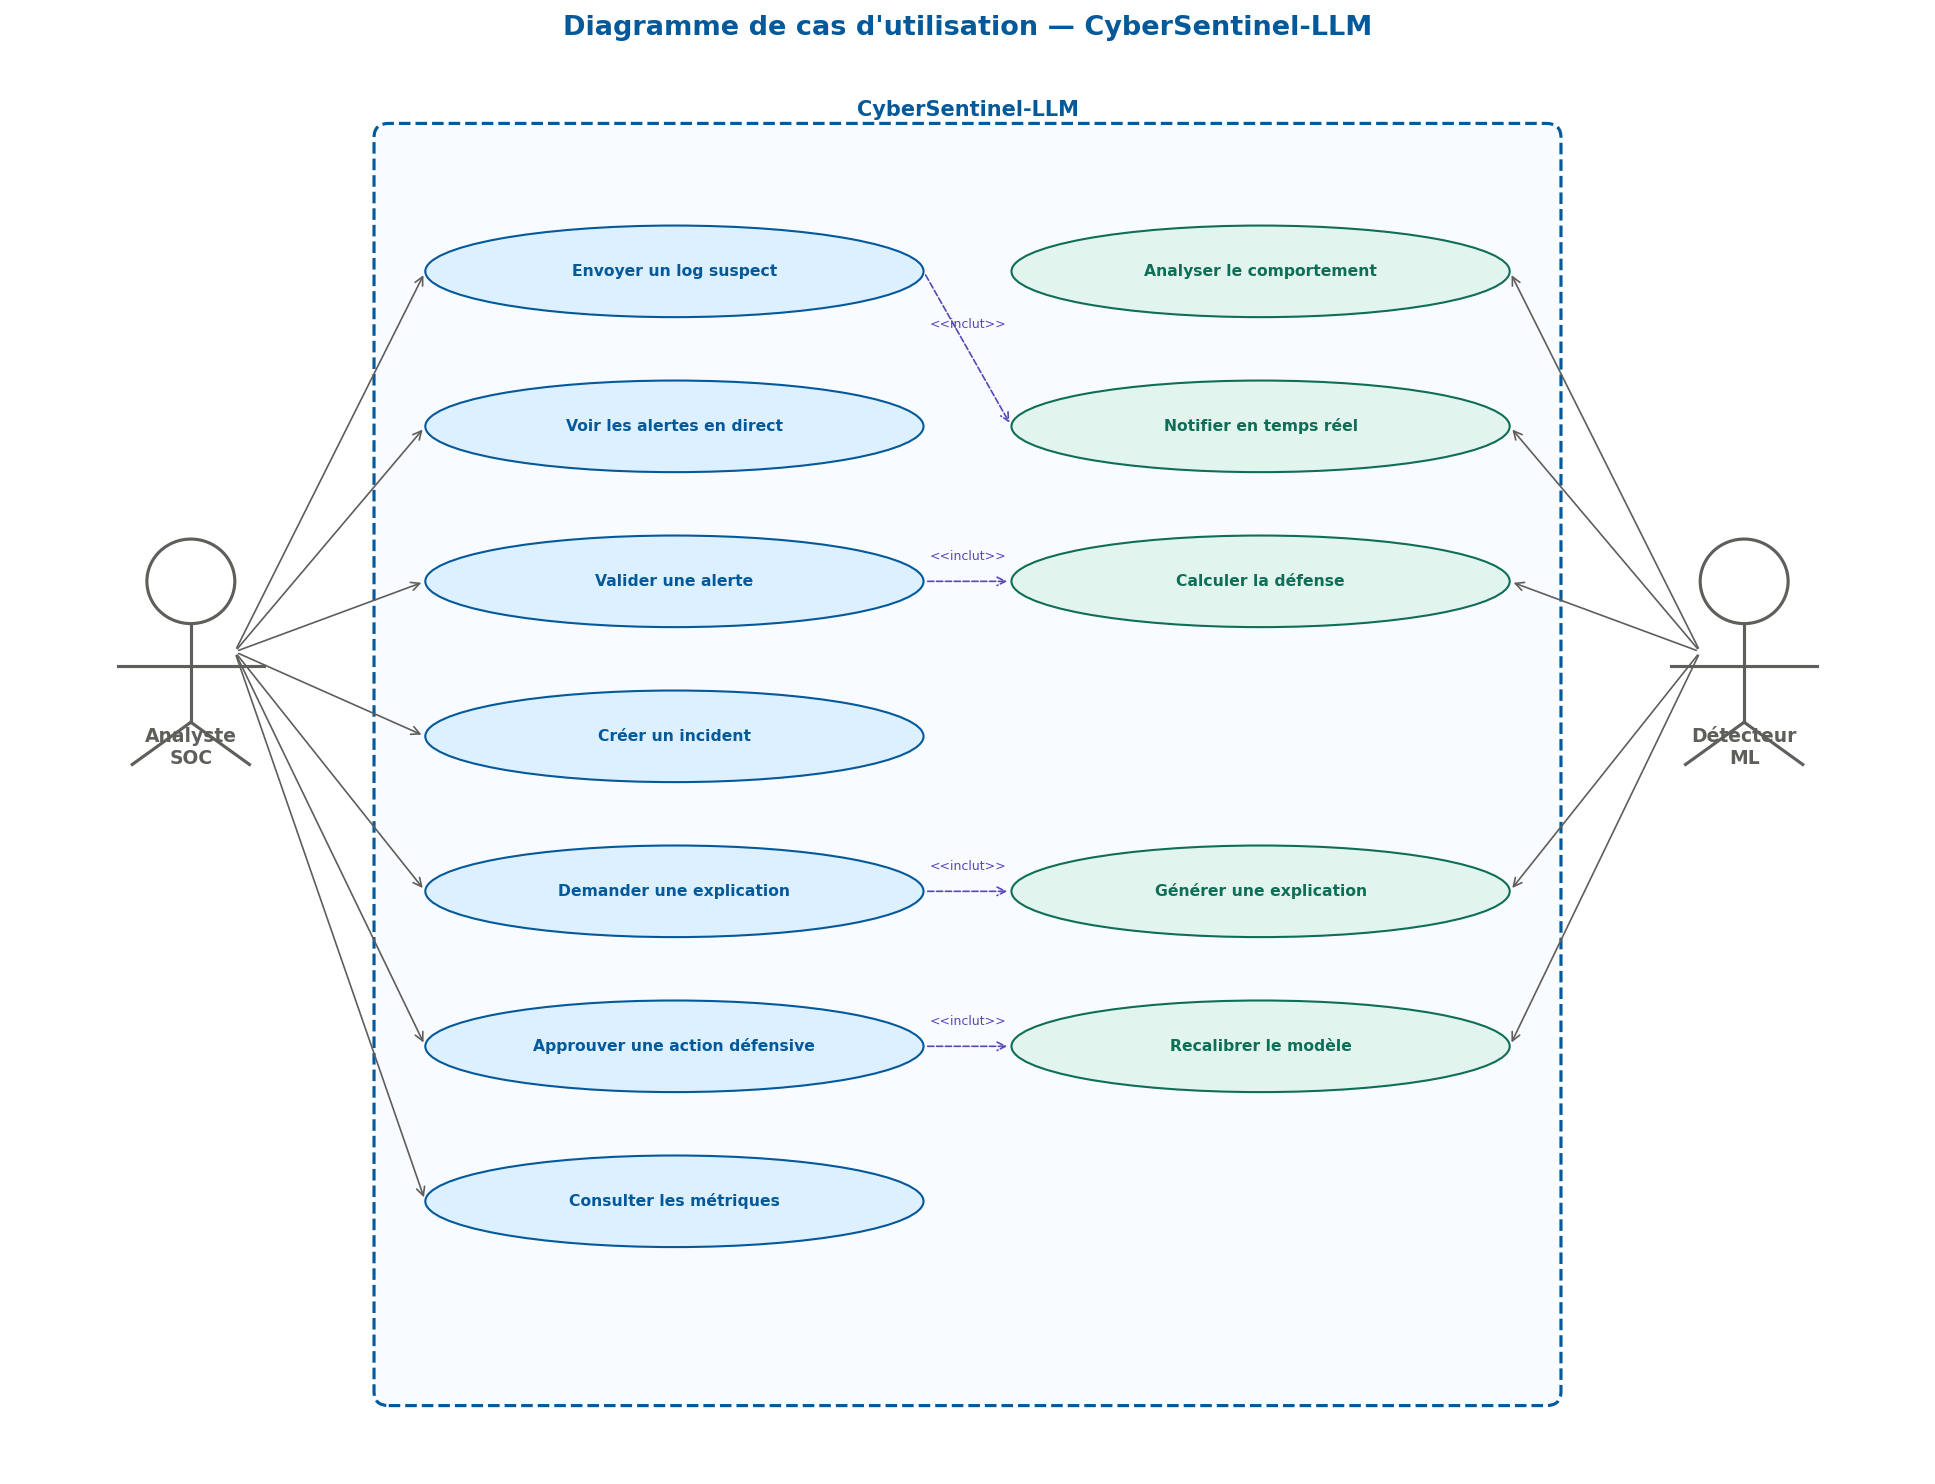
\includegraphics[width=0.90\linewidth]{images/cybersentinel_use_case.png}
\caption{Diagramme de cas d'utilisation de CyberSentinel-LLM}
\label{fig:usecase}
\end{figure}

\section{Exigences fonctionnelles}
\begin{onehalfspace}
Les exigences fonctionnelles définissent les fonctionnalités que le système
doit obligatoirement implémenter :
\end{onehalfspace}

\begin{table}[!h]
\centering
\caption{Exigences fonctionnelles de CyberSentinel-LLM}
\begin{tabular}{|p{1cm}|p{4cm}|p{8.5cm}|}
\hline
\textbf{ID} & \textbf{Fonctionnalité} & \textbf{Description} \\
\hline
EF01 & Ingestion de logs & Recevoir et traiter 1..N logs via POST /ingest/logs \\
\hline
EF02 & Scoring ML & Calculer un score d'anomalie 0..1 par log ingéré (IF/LOF/hybride) \\
\hline
EF03 & Gestion des alertes & Lister, filtrer et labelliser les alertes générées \\
\hline
EF04 & Gestion des incidents & Créer, consulter et suivre les incidents \\
\hline
EF05 & RAG MITRE ATT\&CK & Indexer 15 techniques et enrichir le contexte LLM \\
\hline
EF06 & Explication LLM & Générer une explication JSON structurée d'un incident \\
\hline
EF07 & Score de confiance & Calculer confidence = 0.4×ML + 0.3×RAG + 0.3×LLM \\
\hline
EF08 & Neutralisation adaptive & Blocage applicatif middleware avec liste noire mémoire \\
\hline
EF09 & Notification blocage & Afficher countdown 30s et demander approbation humaine \\
\hline
EF10 & Chat conversationnel & Interface de chat avec le LLM local (texte + voix) \\
\hline
EF11 & Streaming temps réel & Diffuser les alertes en temps réel via SSE \\
\hline
EF12 & Cartographie GeoIP & Afficher la localisation géographique des IPs sources \\
\hline
EF13 & Métriques ML & Calculer et afficher precision/recall/F1/roc\_auc \\
\hline
\end{tabular}
\end{table}

\section{Exigences non fonctionnelles}
\begin{onehalfspace}
Les exigences non fonctionnelles définissent les contraintes de qualité,
de performance et de sécurité du système :

\begin{itemize}
  \item[\ding{43}] \textbf{Réplicabilité locale :} le système doit être
  entièrement déployable sur une machine locale sans dépendance à des
  services cloud (Ollama local, SQLite, ChromaDB local) ;
  \item[\ding{43}] \textbf{Compatibilité matérielle contrainte :} toute la
  chaîne de traitement (ML + embedding RAG + LLM) doit fonctionner sur CPU
  Intel i7 11\textsuperscript{ème} génération avec 16 GB de RAM, sans GPU ;
  \item[\ding{43}] \textbf{Performance minimale :} le scoring ML doit
  s'exécuter en moins de 50 ms par alerte ; l'explication LLM est tolérée
  entre 30 et 90 secondes sur CPU ;
  \item[\ding{43}] \textbf{Sécurité minimale :} CORS configurable,
  rate limiting par IP, security headers HTTP, limitation de taille
  des requêtes ;
  \item[\ding{43}] \textbf{Maintenabilité :} architecture modulaire
  (routers / services / models) facilitant l'extension et la maintenance ;
  \item[\ding{43}] \textbf{Principe Human-in-the-Loop :} le LLM ne prend
  aucune décision autonome sur le système ; toute action défensive de
  type blocage requiert une approbation humaine explicite.
\end{itemize}
\end{onehalfspace}

\section*{Conclusion du Chapitre 2}
\addcontentsline{toc}{section}{Conclusion}
\begin{onehalfspace}
Ce chapitre a défini les cas d'usage, les exigences fonctionnelles et
non fonctionnelles de \textbf{CyberSentinel-LLM}. Ces spécifications
guideront la conception architecturale et l'implémentation détaillée
présentées dans les chapitres suivants.
\end{onehalfspace}

\newpage

%% ============================================================
%% CHAPITRE 3
%% ============================================================
\chapter{Conception Logicielle et Architecture}

\section*{Introduction}
\addcontentsline{toc}{section}{Introduction}
\begin{onehalfspace}
Ce chapitre présente l'architecture globale de \textbf{CyberSentinel-LLM},
la structure du code, la description détaillée des composants backend et
frontend, ainsi que les diagrammes UML illustrant les flux et les interactions
entre les différents modules du système.
\end{onehalfspace}

\section{Architecture globale}
\begin{onehalfspace}
\textbf{CyberSentinel-LLM} repose sur une \textbf{architecture monolithique
modulaire orientée API en cinq couches}. Ce choix architectural garantit la
simplicité du déploiement local tout en permettant une séparation claire des
responsabilités entre les composantes du système.\\

L'architecture comprend cinq grandes couches :
\begin{itemize}
  \item[\ding{43}] \textbf{Couche 1 — Frontend (UI) :} interface Next.js 16
  (App Router), 9 pages SOC (dashboard, alertes, incidents, demo, chat,
  modèle ML, paramètres, rapports, login), intégration SSE et WebSocket ;
  \item[\ding{43}] \textbf{Couche 2 — API Gateway :} FastAPI modulaire avec
  routers, endpoints, middlewares de sécurité et middleware de blocage IP ;
  \item[\ding{43}] \textbf{Couche 3 — Détection ML :} pipeline non supervisé
  + heuristique (IsolationForest, LOF, fallback), scoring 0..1, règles de
  sévérité ;
  \item[\ding{43}] \textbf{Couche 4 — RAG + LLM :} ChromaDB avec 15
  techniques MITRE ATT\&CK, embedding all-MiniLM-L6-v2, Ollama pour
  explication structurée et chat conversationnel ;
  \item[\ding{43}] \textbf{Couche 5 — Défense :} moteur de décision
  défensive, liste noire mémoire O(1), middleware blocage IP (HTTP 403),
  génération commandes iptables.
\end{itemize}
\end{onehalfspace}

\begin{figure}[!h]
\centering
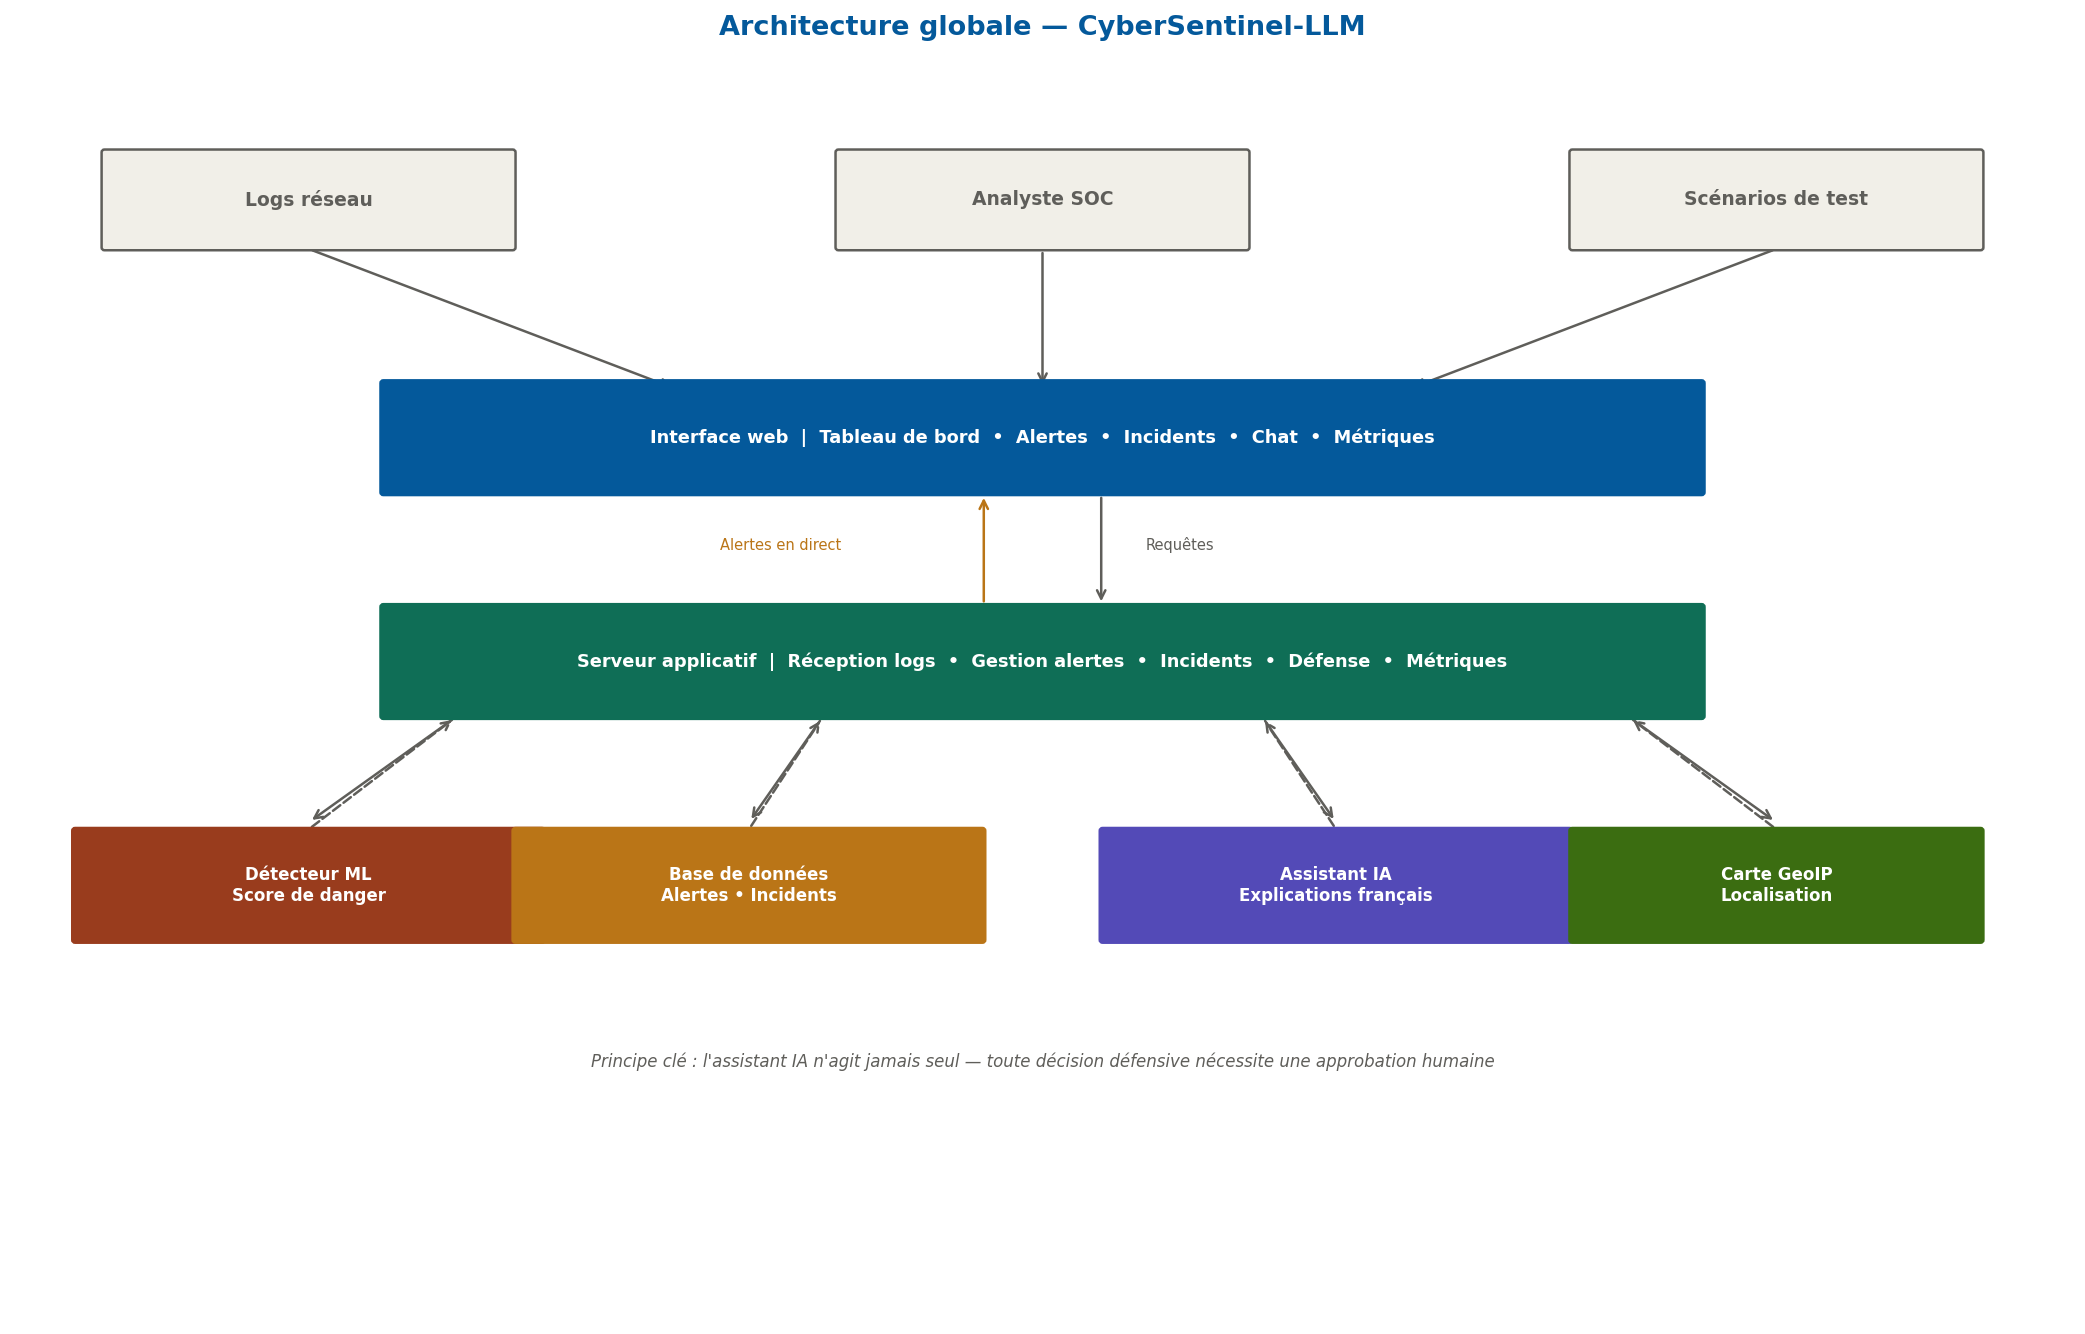
\includegraphics[width=0.90\linewidth]{images/cybersentinel_architecture.png}
\caption{Architecture globale de CyberSentinel-LLM}
\label{fig:architecture}
\end{figure}

\section{Arborescence du projet}
\begin{onehalfspace}
Le projet est organisé selon la structure suivante :
\end{onehalfspace}

\begin{tcolorbox}[colback=lightblue, colframe=darkblue, arc=5pt,
  title={\textbf{Structure du projet CyberSentinel-LLM}}]
\begin{small}
\begin{verbatim}
cybersentinel-llm/
|-- backend/
|   |-- app/
|   |   |-- core/           # Configuration et settings
|   |   |-- db/             # Connexion base de donnees
|   |   |-- routers/        # Contrats API metier
|   |   |-- endpoints/      # Endpoints LLM avances (chat, TTS, STT)
|   |   |-- models/         # Entites SQLModel (8 tables)
|   |   `-- services/       # Logique technique transverse
|   |       |-- detection.py    # ML : IF, LOF, heuristique
|   |       |-- rag_service.py  # ChromaDB + MITRE ATT&CK
|   |       |-- llm_ollama.py   # Ollama + RAG + confiance
|   |       |-- ip_blacklist.py # Liste noire memoire
|   |       |-- defense.py      # Moteur decision defensive
|   |       |-- geoip.py        # Lookup MaxMind GeoLite2
|   |       |-- sse.py          # Server-Sent Events
|   |       |-- tts_service.py  # Synthese vocale Piper
|   |       `-- whisper_service.py  # Transcription Whisper
|-- frontend/
|   |-- app/
|   |   |-- dashboard/      # Vue temps reel
|   |   |-- alerts/         # Gestion alertes + blocage
|   |   |-- incidents/      # Incidents + explication LLM
|   |   |-- demo/           # Pipeline 5 etapes anime
|   |   |-- chat/           # Chat SOC texte + voix
|   |   |-- model/          # Metriques ML
|   |   |-- settings/       # Parametres + IPs bloquees
|   |   |-- reports/        # Rapports + export CSV
|   |   `-- login/          # Authentification
|   `-- components/
|       |-- BlockingNotification.tsx  # Notification blocage
|       |-- WorldMap.tsx              # Carte GeoIP Leaflet
|       `-- ...
`-- chroma_db/              # Persistance ChromaDB locale
\end{verbatim}
\end{small}
\end{tcolorbox}

\section{Description des composants backend}
\begin{onehalfspace}
Le backend est organisé en modules distincts, chacun ayant une responsabilité
clairement définie :
\end{onehalfspace}

\begin{table}[!h]
\centering
\caption{Description des composants backend}
\begin{tabular}{|p{5cm}|p{8.5cm}|}
\hline
\textbf{Composant} & \textbf{Rôle} \\
\hline
\texttt{services/detection.py} & Extraction de 5 features, entraînement
IF/LOF, scoring 0..1, fallback heuristique \\
\hline
\texttt{services/rag\_service.py} & ChromaDB, embedding all-MiniLM-L6-v2,
15 techniques MITRE ATT\&CK, retrieve\_context() \\
\hline
\texttt{services/llm\_ollama.py} & Prompt RAG enrichi, appel Ollama,
parsing JSON, retry, confiance pondérée \\
\hline
\texttt{services/ip\_blacklist.py} & Liste noire mémoire thread-safe,
synchronisation DB, boucle d'expiration \\
\hline
\texttt{services/defense.py} & Moteur de décision défensive (4 modes),
TTL blocage \\
\hline
\texttt{services/geoip.py} & Lookup MaxMind GeoLite2-City.mmdb \\
\hline
\texttt{services/sse.py} & Queues asyncio multi-abonnés, publication
alertes temps réel \\
\hline
\texttt{services/tts\_service.py} & Synthèse vocale Piper locale \\
\hline
\texttt{services/whisper\_service.py} & Transcription vocale STT locale \\
\hline
\texttt{routers/ingest.py} & Ingestion logs, scoring ML, GeoIP, SSE \\
\hline
\texttt{routers/defense.py} & Endpoints approve/revoke/block-manual \\
\hline
\texttt{routers/metrics.py} & Calcul precision/recall/F1/roc\_auc \\
\hline
\texttt{models/} & Alert, Incident, LLMTrace, IPEnrichment, AlertLabel,
Conversation, ChatMessage, DefenseAction \\
\hline
\end{tabular}
\end{table}

\section{Description du frontend}
\begin{onehalfspace}
Le frontend est développé avec \textbf{Next.js 16} (App Router) en mode
dark cybersécurité et offre une interface SOC complète en 9 pages :

\begin{itemize}
  \item[\ding{43}] \textbf{/dashboard :} vue temps réel avec 4 KPIs, timeline
  24h, distribution sévérité, carte GeoIP, 10 dernières alertes, badge LIVE ;
  \item[\ding{43}] \textbf{/alerts :} liste complète des alertes, labellisation
  (true\_attack / false\_positive), approbation/révocation des blocages ;
  \item[\ding{43}] \textbf{/incidents/[id] :} détail d'un incident, explication
  LLM enrichie RAG, techniques MITRE identifiées, décision humaine ;
  \item[\ding{43}] \textbf{/demo :} pipeline IDS 5 étapes animé avec terminal
  live, carte GeoIP, explication LLM et blocage automatisé ;
  \item[\ding{43}] \textbf{/chat :} console conversationnelle streaming avec
  historique persisté, mode voix (STT Whisper + TTS Piper) ;
  \item[\ding{43}] \textbf{/model :} métriques ML (F1-score, précision,
  rappel, ROC-AUC, seuil actif) ;
  \item[\ding{43}] \textbf{/settings :} état des services, gestion des IPs
  bloquées, blocage manuel, commandes iptables actives ;
  \item[\ding{43}] \textbf{/reports :} statistiques par période, top
  attaquants, distribution MITRE, export CSV/TXT ;
  \item[\ding{43}] \textbf{/login :} authentification et inscription.
\end{itemize}
\end{onehalfspace}

\section{Diagrammes UML}

\subsection{Diagramme de classes}
\begin{figure}[!h]
\centering
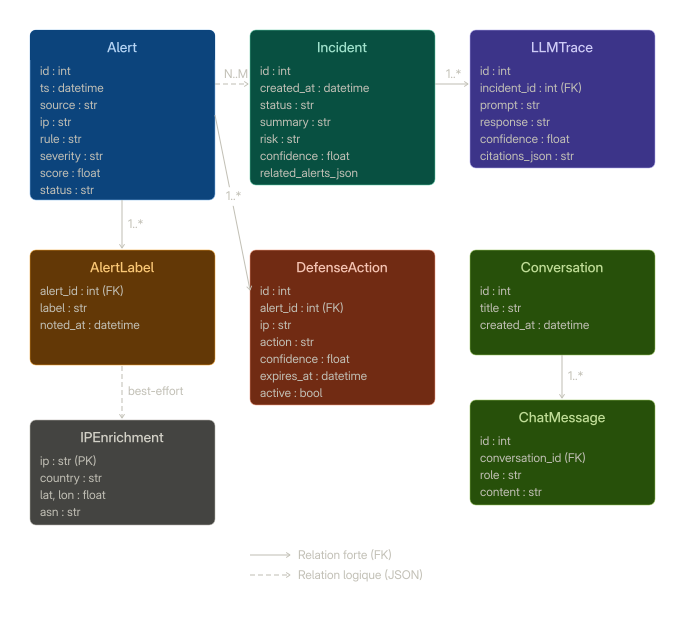
\includegraphics[width=0.90\linewidth]{images/cybersentinel_class_diagram.png}
\caption{Diagramme de classes de CyberSentinel-LLM}
\label{fig:classes}
\end{figure}

\subsection{Diagramme de séquence}
\begin{figure}[!h]
\centering
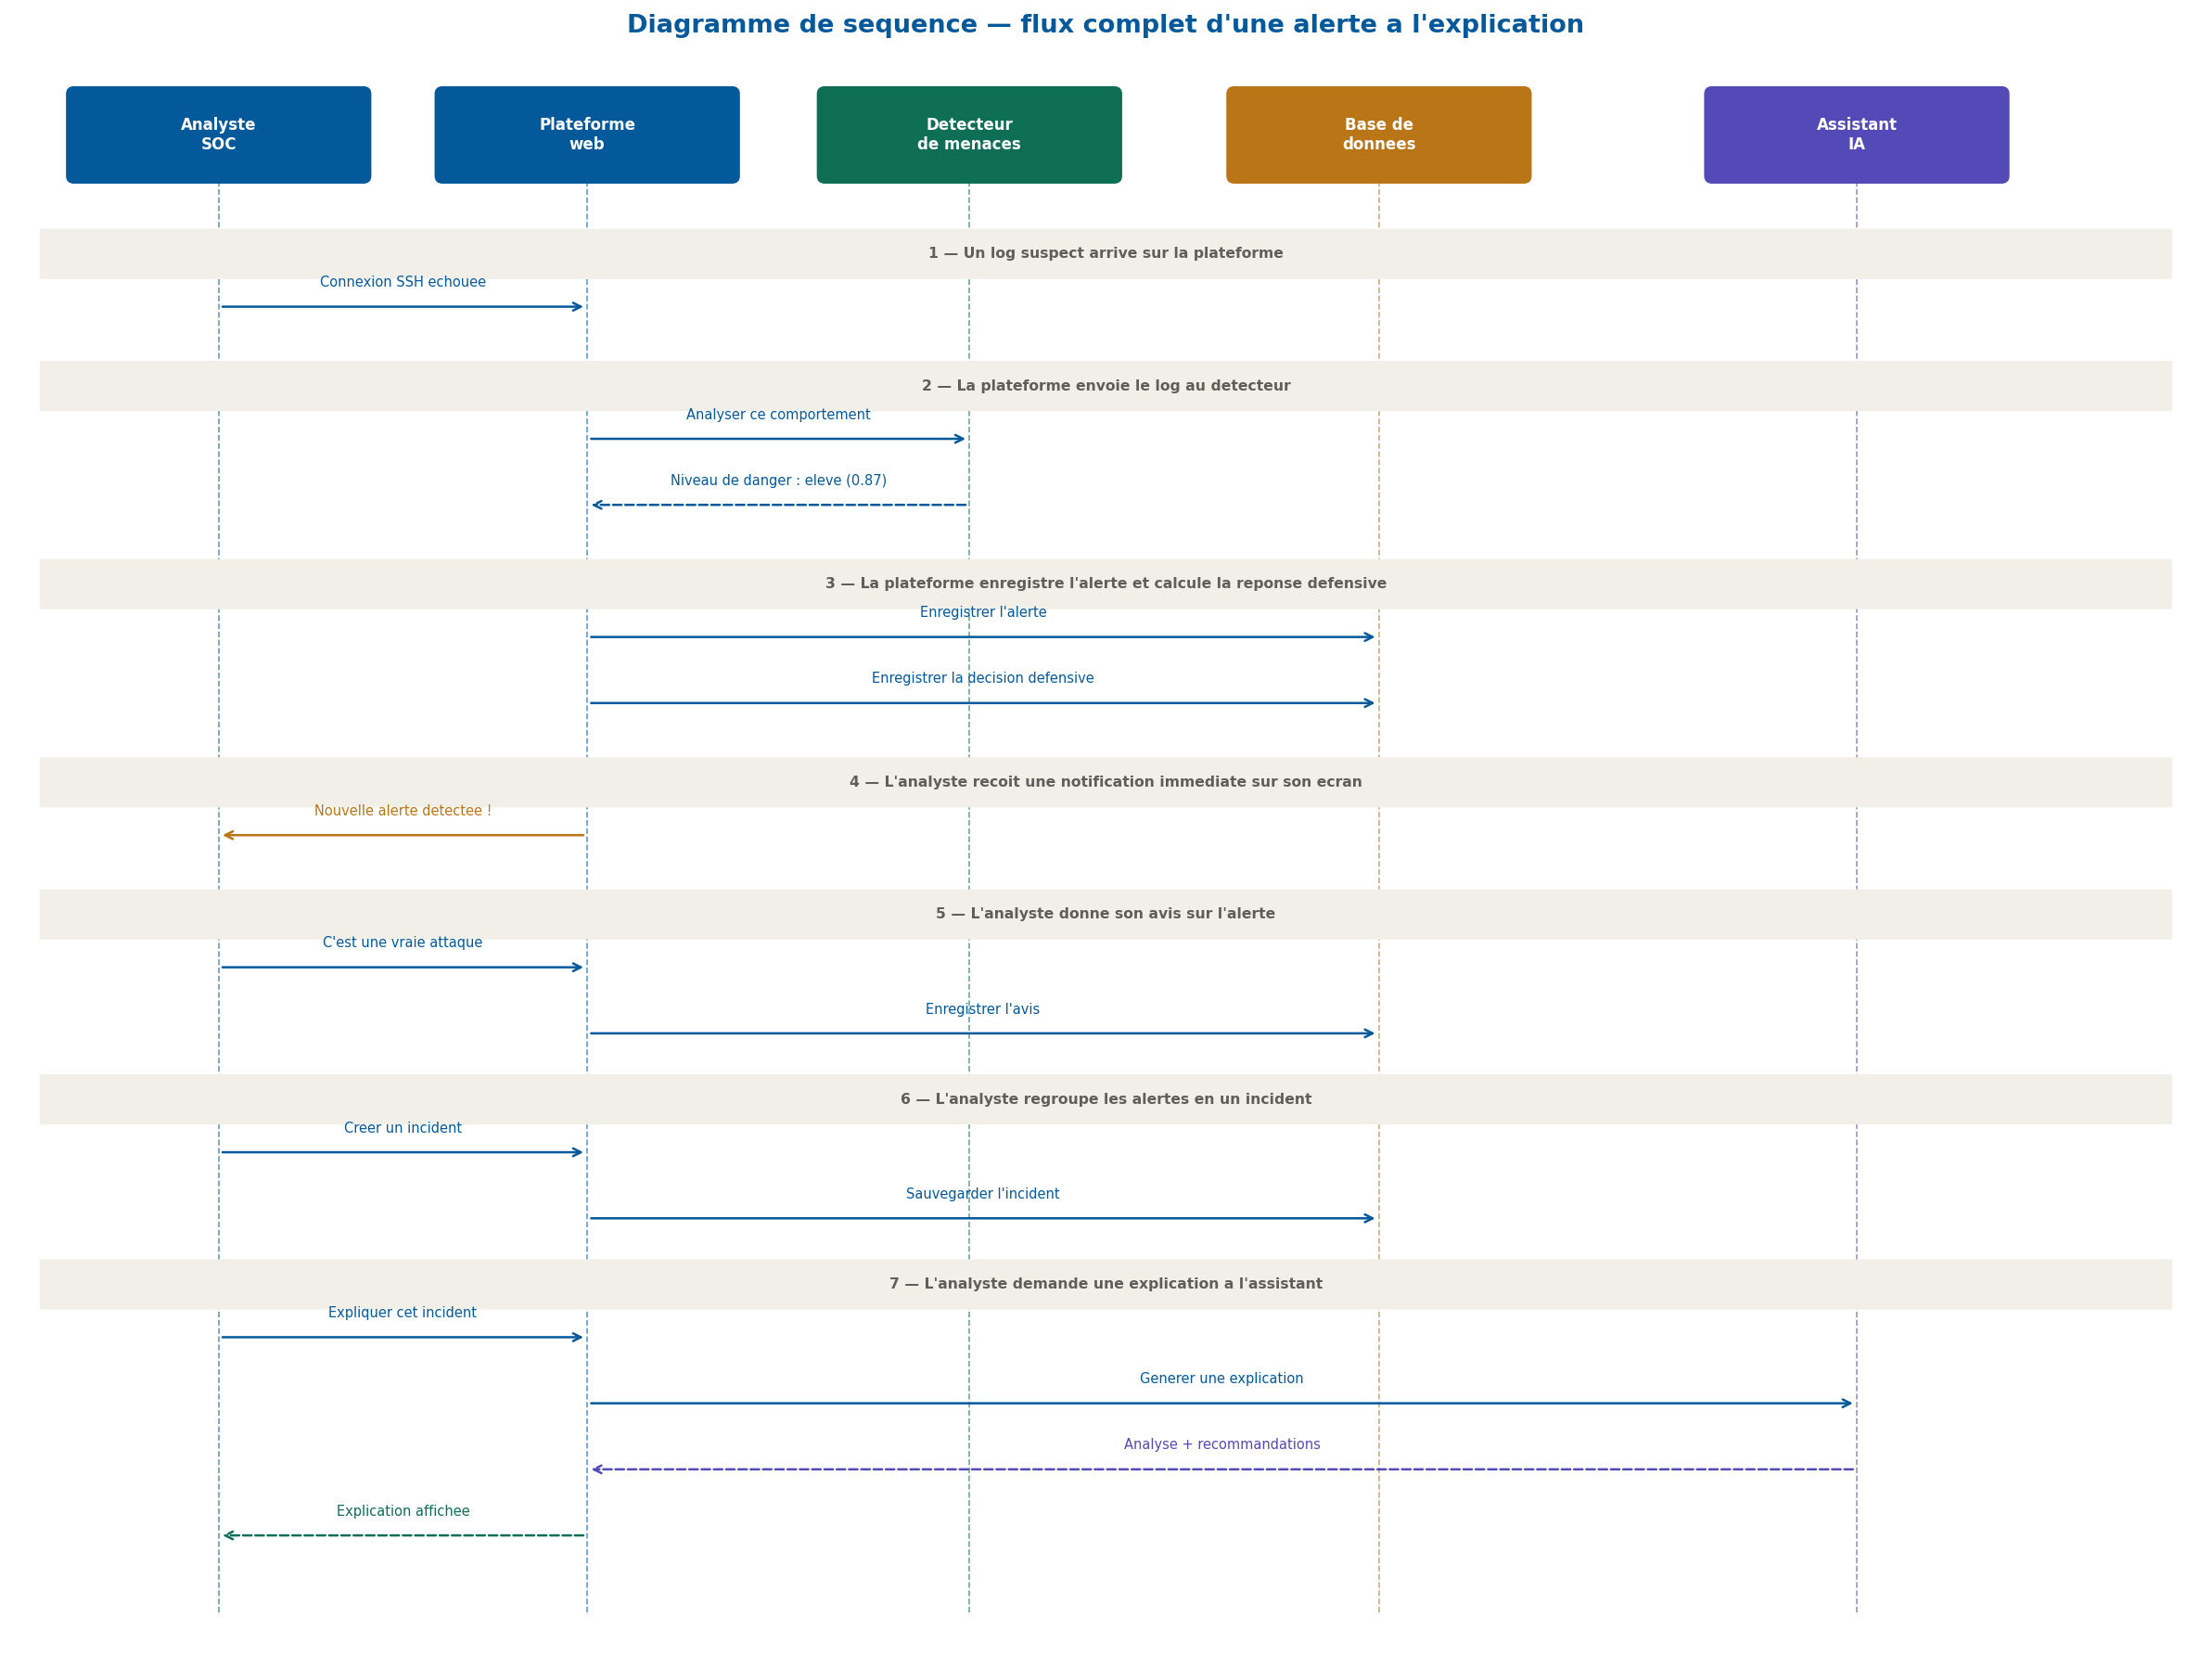
\includegraphics[width=0.90\linewidth]{images/sequence_simplifie_fr.png}
\caption{Diagramme de séquence — flux d'une alerte jusqu'à la neutralisation}
\label{fig:sequence}
\end{figure}

\subsection{Diagramme d'activité}
\begin{figure}[!h]
\centering
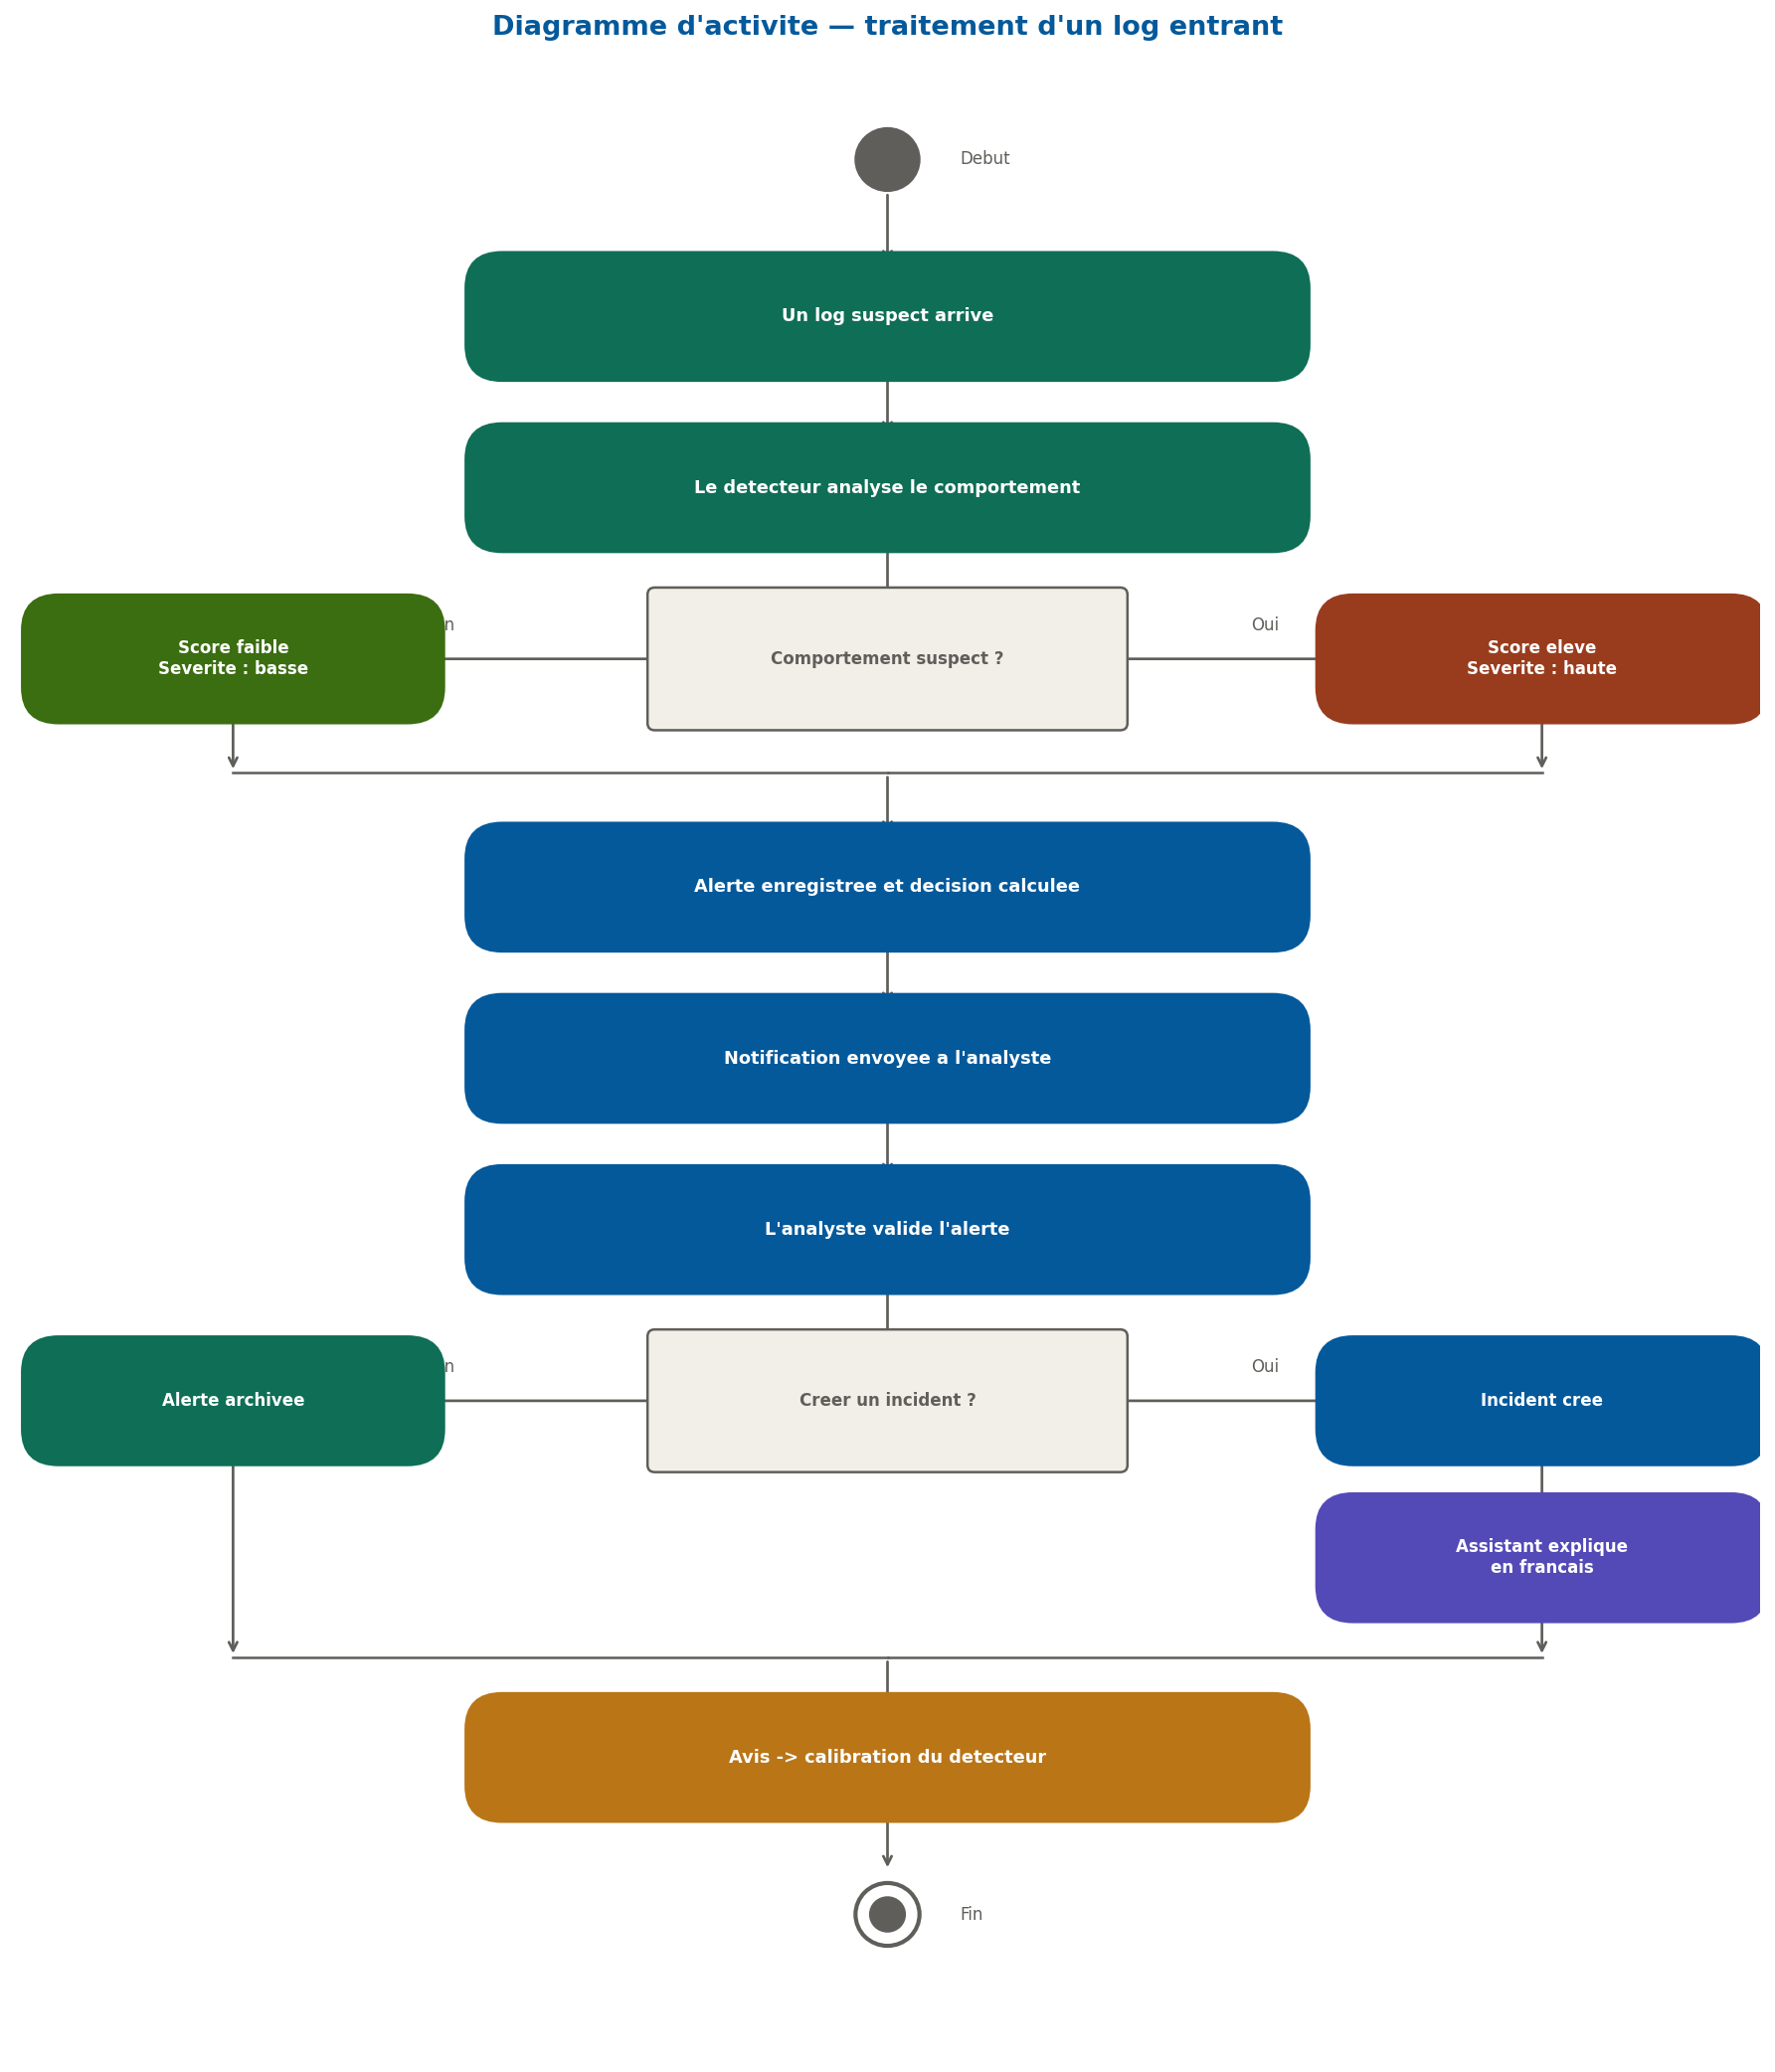
\includegraphics[width=0.75\linewidth]{images/cybersentinel_activity.png}
\caption{Diagramme d'activité — traitement d'un log entrant}
\label{fig:activite}
\end{figure}

\section*{Conclusion du Chapitre 3}
\addcontentsline{toc}{section}{Conclusion}
\begin{onehalfspace}
Ce chapitre a présenté l'architecture globale en cinq couches, la structure
du projet et les composants principaux de \textbf{CyberSentinel-LLM}. Les
diagrammes UML illustrent les flux de données et les interactions entre les
modules. Le chapitre suivant détaillera l'implémentation concrète de chaque
composante.
\end{onehalfspace}

\newpage

%% ============================================================
%% CHAPITRE 4
%% ============================================================
\chapter{Implémentation}

\section*{Introduction}
\addcontentsline{toc}{section}{Introduction}
\begin{onehalfspace}
Ce chapitre présente les détails d'implémentation de \textbf{CyberSentinel-LLM}:
le pipeline ML de détection d'anomalies, le module RAG MITRE ATT\&CK, le module
LLM avec score de confiance pondéré, le système de neutralisation adaptive par
blocage applicatif, la communication en temps réel par SSE, et les endpoints
principaux de l'API.
\end{onehalfspace}

\section{Pipeline Machine Learning}
\begin{onehalfspace}
Le pipeline ML de \textbf{CyberSentinel-LLM} suit les étapes suivantes :

\begin{enumerate}
  \item \textbf{Extraction des features} depuis le log brut (5 features) ;
  \item \textbf{Construction de la matrice d'entraînement} :
  \texttt{\_build\_training\_matrix(N=200)} à partir des 200 dernières alertes ;
  \item \textbf{Scoring} via IF/LOF/hybride selon la variable
  d'environnement \texttt{DETECTOR} ;
  \item \textbf{Application du seuil} \texttt{SCORE\_THRESHOLD} (défaut : 0.6) ;
  \item \textbf{Mapping score $\rightarrow$ sévérité} : high ($\geq$ 0.8),
  medium ($\geq$ 0.5), low (< 0.5).
\end{enumerate}
\end{onehalfspace}

\begin{table}[!h]
\centering
\caption{Features utilisées dans le pipeline ML}
\begin{tabular}{|p{4.5cm}|p{9cm}|}
\hline
\textbf{Feature} & \textbf{Description / Formule} \\
\hline
\texttt{is\_ssh} & 1.0 si source == "ssh", sinon 0.0 \\
\hline
\texttt{is\_fail} & 1.0 si status == "fail", sinon 0.0 \\
\hline
\texttt{hour\_sin} & $\sin(2\pi \times (h + m/60) / 24)$ \\
\hline
\texttt{hour\_cos} & $\cos(2\pi \times (h + m/60) / 24)$ \\
\hline
\texttt{ip\_fail\_count\_60m} & Nombre d'alertes fail pour cette IP sur 60 min (SQLite) \\
\hline
\end{tabular}
\end{table}

\begin{onehalfspace}
\textbf{Scoring IsolationForest :} le score décisionnel brut est transformé
via une fonction sigmoïde inverse :
\end{onehalfspace}

\begin{tcolorbox}[colback=lightblue, colframe=darkblue, arc=5pt,
  title={\textbf{Formule IsolationForest}}]
\[
P_{normal} = \frac{1}{1 + e^{-k \cdot df}}, \quad k=4 \qquad
score_{IF} = 1 - P_{normal} \in [0, 1]
\]
\end{tcolorbox}

\begin{onehalfspace}
\textbf{Scoring LOF :} le facteur d'anomalie local est normalisé par
min-max sur le batch :
\end{onehalfspace}

\begin{tcolorbox}[colback=lightblue, colframe=darkblue, arc=5pt,
  title={\textbf{Formule LOF normalisée}}]
\[
score_{LOF} = 1 - \frac{nof_x - nof_{min}}{nof_{max} - nof_{min}}
\]
\end{tcolorbox}

\begin{onehalfspace}
\textbf{Mode hybride :} $score = \max(score_{IF}, score_{LOF})$\\[6pt]
\textbf{Fallback heuristique} (< 20 échantillons en base) :
\end{onehalfspace}

\begin{tcolorbox}[colback=lightblue, colframe=darkblue, arc=5pt,
  title={\textbf{Formule de fallback heuristique}}]
\[
score = 0.2 + 0.5 \times is\_fail + \min(ip\_fail\_count, 5) \times 0.05
\]
\end{tcolorbox}

\section{Module RAG — MITRE ATT\&CK}
\begin{onehalfspace}
Le module RAG constitue une contribution centrale de \textbf{CyberSentinel-LLM}.
Il permet au LLM de raisonner sur des références cybersécurité précises plutôt
que sur sa seule mémoire d'entraînement.

\subsection*{Architecture ChromaDB}
\begin{itemize}
  \item[\ding{43}] \textbf{Collection :} \texttt{mitre\_attack}, distance cosinus
  (\texttt{hnsw:space: cosine}) ;
  \item[\ding{43}] \textbf{Persistance :} dossier \texttt{chroma\_db/} à la
  racine du projet ;
  \item[\ding{43}] \textbf{Initialisation idempotente :} ne réindexe que si
  la collection est vide — aucune pénalité au redémarrage ;
  \item[\ding{43}] \textbf{Modèle d'embedding :} \textit{all-MiniLM-L6-v2}
  (sentence-transformers, $\sim$80 MB, CPU-only, 384 dimensions).
\end{itemize}

\subsection*{Techniques MITRE ATT\&CK indexées}
\end{onehalfspace}

\begin{table}[!h]
\centering
\caption{15 techniques MITRE ATT\&CK indexées dans ChromaDB}
\begin{tabular}{|p{2.5cm}|p{5cm}|p{1.5cm}|}
\hline
\textbf{ID} & \textbf{Nom} & \textbf{Sévérité} \\
\hline
T1110.001 & Password Guessing (Brute Force SSH) & high \\
\hline
T1110.003 & Password Spraying & high \\
\hline
T1078 & Valid Accounts & high \\
\hline
T1021.004 & SSH Remote Services & medium \\
\hline
T1059.004 & Unix Shell & high \\
\hline
T1190 & Exploit Public-Facing Application & high \\
\hline
T1046 & Network Service Discovery & medium \\
\hline
T1595.001 & Scanning IP Blocks & medium \\
\hline
T1133 & External Remote Services & medium \\
\hline
T1071.001 & Web Protocols (C2) & high \\
\hline
T1048 & Exfiltration Over Alternative Protocol & high \\
\hline
T1098 & Account Manipulation & high \\
\hline
T1136 & Create Account & medium \\
\hline
T1070.003 & Clear Command History & medium \\
\hline
T1562.001 & Disable Security Tools & high \\
\hline
\end{tabular}
\end{table}

\begin{onehalfspace}
\textbf{Score de pertinence RAG :} la similarité cosinus est calculée depuis
la distance ChromaDB :

\begin{tcolorbox}[colback=lightblue, colframe=darkblue, arc=5pt,
  title={\textbf{Score de pertinence RAG}}]
\[
similarity_{RAG} = \max\!\left(0,\, \min\!\left(1,\, 1 - \frac{distance}{2}\right)\right)
\quad \in [0, 1]
\]
\end{tcolorbox}
\end{onehalfspace}

\section{Module LLM et Score de Confiance}
\begin{onehalfspace}
Le module LLM est au cœur de la valeur ajoutée de \textbf{CyberSentinel-LLM}.
Il intègre le contexte RAG pour produire des explications fondées et traçables.

\subsection*{Modèle utilisé}
Modèle : \textit{qwen2.5:1.5b} via Ollama local (\texttt{http://localhost:11434}),
avec sortie JSON forcée (\texttt{"format": "json"}).

\begin{onehalfspace}
\textbf{Optimisations pour inférence CPU :} afin de garantir
des temps de réponse acceptables (30--90 secondes sur CPU sans GPU),
plusieurs paramètres ont été configurés :

\begin{itemize}
  \item[\ding{43}] \texttt{keep\_alive: -1} — maintient le modèle
  chargé en RAM entre les requêtes, évitant le rechargement
  coûteux à chaque appel ;
  \item[\ding{43}] \texttt{num\_predict: 600} — limite la longueur
  de la réponse générée pour réduire le temps d'inférence ;
  \item[\ding{43}] \texttt{num\_ctx: 2048} — fenêtre de contexte
  adaptée aux prompts RAG enrichis ;
  \item[\ding{43}] \texttt{temperature: 0.1} — sortie déterministe
  favorisant des réponses JSON stables et parsables ;
  \item[\ding{43}] \textbf{Warm-up au démarrage} — un appel initial
  au démarrage du serveur précharge le modèle en RAM.
\end{itemize}
\end{onehalfspace}

\subsection*{Prompt template RAG enrichi}
\end{onehalfspace}

\begin{tcolorbox}[colback=lightblue, colframe=darkblue, arc=5pt,
  title={\textbf{Template de prompt RAG — Explication d'incident}}]
\begin{small}
\begin{verbatim}
Tu es un expert SOC spécialisé en cybersécurité.

Contexte MITRE ATT&CK récupéré automatiquement :
{rag_context}

Incident à analyser : {incident_summary}
Alertes associées : {alert_ids}

Réponds UNIQUEMENT avec un objet JSON valide :
{
  "severity_score": <entier 0-10>,
  "attack_type": "<nom court en français>",
  "mitre_technique": "<ID ex: T1110.001>",
  "mitre_name": "<nom de la technique>",
  "explanation": "<2-3 phrases en français>",
  "recommended_actions": ["action1", "action2", "action3"],
  "confidence_score": <float 0.0-1.0>,
  "confidence_justification": "<justification>"
}
\end{verbatim}
\end{small}
\end{tcolorbox}

\begin{onehalfspace}
\textbf{Mécanisme de retry :} en cas d'échec du parsing JSON, le système
effectue une nouvelle tentative avec un prompt simplifié, puis utilise un
JSON de fallback statique (confidence = 0.2, méthode = "fallback").\\[6pt]

\textbf{Formule de confiance pondérée :} le score de confiance final est
calculé comme une moyenne pondérée de trois sources indépendantes :
\end{onehalfspace}

\begin{tcolorbox}[colback=lightblue, colframe=darkblue, arc=5pt,
  title={\textbf{Formule de confiance pondérée}}]
\[
confidence_{final} = 0.4 \times score_{ML} + 0.3 \times similarity_{RAG}
+ 0.3 \times score_{LLM}
\]
\end{tcolorbox}

\begin{onehalfspace}
Où $score_{ML} \in [0,1]$ est le score IsolationForest/LOF, $similarity_{RAG}
\in [0,1]$ est la similarité cosinus de la meilleure correspondance MITRE,
et $score_{LLM} \in [0,1]$ est le score de confiance retourné par le LLM
dans son JSON.
\end{onehalfspace}

\section{Système de Neutralisation Adaptive}
\begin{onehalfspace}
Le système de neutralisation adaptive constitue la contribution la plus
innovante de \textbf{CyberSentinel-LLM} sur le plan opérationnel. Il
implémente un IDS/IPS hybride à validation humaine.

\subsection*{Les quatre modes de défense}
\end{onehalfspace}

\begin{table}[!h]
\centering
\caption{Modes de défense du module de neutralisation}
\begin{tabular}{|p{2.5cm}|p{4cm}|p{7cm}|}
\hline
\textbf{Mode} & \textbf{Comportement} & \textbf{Action produite} \\
\hline
\texttt{off} & Aucune action & allow — passive uniquement \\
\hline
\texttt{monitor} & Surveillance seule & monitor — log uniquement \\
\hline
\texttt{assist} & Aide humaine (défaut) & review si score $\geq$ 0.60 ;
block\_temp si règle connue + high \\
\hline
\texttt{auto} & Blocage automatique & block\_temp si score $\geq$ 0.85,
sans validation humaine \\
\hline
\end{tabular}
\end{table}

\begin{onehalfspace}
\textbf{Middleware de blocage (main.py) :} un middleware FastAPI intercepte
chaque requête entrante et retourne HTTP 403 si l'IP source est dans la liste
noire mémoire, avec la commande iptables correspondante :
\end{onehalfspace}

\begin{tcolorbox}[colback=lightblue, colframe=darkblue, arc=5pt,
  title={\textbf{Réponse HTTP 403 — IP bloquée}}]
\begin{small}
\begin{verbatim}
{
  "error": "IP temporairement bloquée",
  "ip": "203.0.113.5",
  "expires_at": "2025-04-09T14:30:00",
  "reason": "known_attack:ssh_failed_login",
  "iptables_command": "iptables -A INPUT -s 203.0.113.5 -j DROP"
}
\end{verbatim}
\end{small}
\end{tcolorbox}

\begin{onehalfspace}
\textbf{Flux de neutralisation complet :}
\end{onehalfspace}

\begin{tcolorbox}[colback=lightblue, colframe=darkblue, arc=5pt,
  title={\textbf{Flux : Détection $\rightarrow$ Notification $\rightarrow$ Blocage}}]
\begin{small}
\begin{verbatim}
1. Alerte créée (score élevé, sévérité high)
2. decide_defense_action() → block_temp recommandé
3. DefenseAction persistée en SQLite
4. SSE → frontend reçoit l'alerte en temps réel
5. BlockingNotification affiche (cas review ET block_temp pending) :
   - IP source + pays de provenance
   - Type d'attaque + technique MITRE
   - Countdown 30 secondes
   - [APPROUVER] / [REJETER]   (raccourci: Esc pour fermer)
6. Analyste approuve → POST /defense/actions/{id}/approve
7. ip_blacklist.add_ip() → liste noire mémoire O(1)
8. Middleware bloque toutes requêtes de cette IP (HTTP 403)
9. Commande iptables affichée pour blocage réseau optionnel
10. Toast de confirmation : « IP bloquee par <analyste> »
\end{verbatim}
\end{small}
\end{tcolorbox}

\begin{onehalfspace}
Les commandes iptables sont générées automatiquement et affichées à
l'analyste pour une application manuelle sur le pare-feu réseau :
\end{onehalfspace}

\begin{tcolorbox}[colback=lightblue, colframe=darkblue, arc=5pt,
  title={\textbf{Commandes iptables générées}}]
\begin{small}
\begin{verbatim}
# Blocage
iptables -A INPUT -s {ip} -j DROP

# Déblocage
iptables -D INPUT -s {ip} -j DROP
\end{verbatim}
\end{small}
\end{tcolorbox}

\section{Endpoints principaux de l'API}
\begin{onehalfspace}
L'API de \textbf{CyberSentinel-LLM} expose un ensemble d'endpoints REST
organisés par domaine fonctionnel :
\end{onehalfspace}

\begin{table}[!h]
\centering
\caption{Endpoints principaux de l'API CyberSentinel-LLM}
\begin{tabular}{|p{1.5cm}|p{5.5cm}|p{6.5cm}|}
\hline
\textbf{Méthode} & \textbf{Endpoint} & \textbf{Rôle} \\
\hline
GET & /health & État API + DB + Ollama + RAG + GeoLite2 \\
\hline
POST & /ingest/logs & Ingérer logs, scorer, GeoIP, défense, SSE \\
\hline
GET & /alerts & Lister alertes (filtres status, severity) \\
\hline
POST & /incidents/from-alerts & Créer incident depuis liste d'alertes \\
\hline
POST & /llm/incidents/\{id\}/explain & Explication LLM + RAG d'un incident \\
\hline
POST & /llm/chat & Chat global streaming \\
\hline
GET & /stream/alerts & Flux SSE temps réel \\
\hline
GET & /map/points & Points GeoIP enrichis \\
\hline
POST & /demo/generate & Génération 3 scénarios SSH simulés \\
\hline
GET & /metrics/model & Métriques ML (F1/précision/rappel/ROC) \\
\hline
POST & /defense/actions/\{id\}/approve & Approuver blocage → liste noire \\
\hline
POST & /defense/actions/\{id\}/revoke & Révoquer blocage \\
\hline
GET & /defense/blocked & Liste IPs actuellement bloquées \\
\hline
POST & /defense/block-manual & Blocage manuel d'une IP \\
\hline
POST & /validation/alerts/\{id\} & Labelliser une alerte \\
\hline
\end{tabular}
\end{table}

\section{SSE et communication temps réel}
\begin{onehalfspace}
La communication temps réel est assurée par le mécanisme
\textbf{Server-Sent Events (SSE)}. Le backend maintient une liste de
queues \texttt{asyncio.Queue} — une par client connecté. À chaque nouvelle
alerte ingérée, l'événement est publié via \texttt{publish\_alert\_created()}
et diffusé à tous les abonnés. La gestion de backpressure limite chaque queue
à 256 éléments.
\end{onehalfspace}

\section{Architecture frontend temps réel}
\begin{onehalfspace}
Côté frontend, l'ensemble des flux temps réel et du polling périodique est
centralisé dans un \textbf{contexte React unique} (\texttt{RealtimeProvider}),
de manière à éviter la multiplication des connexions \textbf{SSE} et des
requêtes redondantes lorsque plusieurs pages consomment les mêmes données.
Le provider expose quatre responsabilités~:

\begin{itemize}
  \item[\ding{43}] \textbf{Une connexion SSE unique} vers \texttt{/stream/alerts},
  rediffusée aux abonnés via un système de \textit{publish/subscribe} interne
  (\texttt{subscribeToAlerts}). Les pages \textit{Dashboard}, \textit{Alertes},
  \textit{Démo} et le composant \texttt{AlertPulse} se branchent dessus sans
  ouvrir leur propre \texttt{EventSource} ;
  \item[\ding{43}] \textbf{Un polling unique} de \texttt{/defense/actions}
  toutes les 5~secondes, qui alimente la liste des actions défensives en
  attente d'approbation humaine ; cette liste pilote à la fois la
  \texttt{BlockingNotification} et un badge pulsant sur l'item
  \textit{Alertes} de la barre latérale ;
  \item[\ding{43}] \textbf{Un polling de santé} \texttt{/health} toutes les
  15~secondes, qui pilote l'indicateur \textit{Backend connecté / SSE actif}
  visible en bas de la barre latérale ;
  \item[\ding{43}] \textbf{Une API de notifications transitoires}
  (\texttt{pushToast}) consommée par toutes les pages pour confirmer les
  approbations, révocations et erreurs de manière non-bloquante.
\end{itemize}

L'arbre du shell applicatif suit donc le schéma~:
\texttt{ErrorBoundary > RealtimeProvider > \{Sidebar, Pages,
BlockingNotification, ToastStack\}}.

\textbf{Ergonomie Human-in-the-Loop renforcée.} Le bouton
\textit{Approuver} est désormais disponible non seulement pour les actions
\texttt{review}, mais aussi pour les actions \texttt{block\_temp} en attente
d'approbation manuelle, ce qui rend explicite le choix de l'analyste avant
toute mise en liste noire. Les opérations destructrices (réinitialisation de
la démo, purge de la base) sont protégées par une boîte de dialogue de
confirmation accessible (raccourcis Échap / Entrée). Pendant la phase
d'analyse LLM (30 à 90~secondes sur CPU), un panneau dédié affiche
l'avancement avec barre de progression et indicateur d'état pour informer
l'analyste que le système n'est pas figé.

\textbf{Robustesse.} Un \texttt{ErrorBoundary} React enveloppe l'ensemble
de l'arbre des composants : toute erreur non capturée affiche un écran de
récupération (« Réessayer / Recharger ») au lieu d'un écran blanc, ce qui
est essentiel pour une console SOC qui doit rester opérationnelle même en
cas d'incident UI.
\end{onehalfspace}

\section*{Conclusion du Chapitre 4}
\addcontentsline{toc}{section}{Conclusion}
\begin{onehalfspace}
Ce chapitre a détaillé l'implémentation des composantes clés de
\textbf{CyberSentinel-LLM} : pipeline ML, module RAG MITRE ATT\&CK,
module LLM avec confiance pondérée, système de neutralisation adaptive
par blocage applicatif, et API REST. Le chapitre suivant présentera les
résultats des tests et l'évaluation du système.
\end{onehalfspace}

\newpage

%% ============================================================
%% CHAPITRE 5
%% ============================================================
\chapter{Tests, Validation et Résultats}

\section*{Introduction}
\addcontentsline{toc}{section}{Introduction}
\begin{onehalfspace}
Ce chapitre présente les scénarios de démonstration, les mécanismes
d'évaluation et les résultats obtenus lors des tests de
\textbf{CyberSentinel-LLM}. L'objectif est de valider le bon fonctionnement
du système dans son ensemble et d'identifier ses limites actuelles.
\end{onehalfspace}

\section{Scénario de démonstration complet}
\begin{onehalfspace}
Un scénario de démonstration reproductible a été développé sur la page
\texttt{/demo} pour valider le flux complet du système en 5 étapes :

\begin{enumerate}
  \item \textbf{Génération des logs} — \texttt{POST /demo/generate} :
  3 événements réseau sont créés :
  2 alertes SSH échouées depuis des IPs externes (US, AU)
  à sévérité HIGH avec recommandation \texttt{block\_temp},
  et 1 requête HTTP suspecte depuis 203.0.113.5 (JP)
  à sévérité MEDIUM avec action \texttt{review}
  (supervision humaine requise). Les IPs sont automatiquement géolocalisées (US, AU, JP) ;

  \item \textbf{Détection ML} — affichage du résultat du scoring :
  "Critique: 2, Faible: 1 — Score max: 0.800" ;

  \item \textbf{Enrichissement GeoIP} — 3 points apparaissent sur la carte
  Leaflet (CartoDB dark matter) ;

  \item \textbf{Analyse LLM + RAG} — incident créé, \texttt{retrieve\_context()}
  identifie T1110.001, T1110.003, T1078 comme techniques pertinentes.
  Ollama génère : \textit{"Brute Force SSH — T1110.001 — confidence: 0.74"} ;

  \item \textbf{Neutralisation} — approbation automatique des 2 blocages HIGH
  en démo, commandes iptables affichées, middleware HTTP 403 actif ;
  la notification de blocage est déclenchée pour les alertes HIGH
  (\texttt{block\_temp}) et MEDIUM avec action \texttt{review}
  (supervision humaine requise).
\end{enumerate}
\end{onehalfspace}

\section{Mécanismes d'évaluation}
\begin{onehalfspace}
L'évaluation du module ML repose sur les labels humains collectés via
le mécanisme de validation (\texttt{true\_attack} / \texttt{false\_positive}).
\end{onehalfspace}

\begin{table}[!h]
\centering
\caption{Métriques d'évaluation du module de détection}
\begin{tabular}{|p{3.5cm}|p{5cm}|p{5cm}|}
\hline
\textbf{Métrique} & \textbf{Formule} & \textbf{Interprétation} \\
\hline
Précision &
$\frac{VP}{VP + FP}$ &
Proportion d'alertes pertinentes parmi celles émises \\
\hline
Rappel &
$\frac{VP}{VP + FN}$ &
Proportion d'attaques réelles détectées \\
\hline
F1-Score &
$\frac{2 \times P \times R}{P + R}$ &
Moyenne harmonique précision/rappel \\
\hline
ROC-AUC &
Aire sous la courbe ROC &
Performance globale du classifieur \\
\hline
Confiance pondérée &
$0.4 \times s_{ML} + 0.3 \times s_{RAG} + 0.3 \times s_{LLM}$ &
Fiabilité globale de l'analyse \\
\hline
\end{tabular}
\end{table}

\section{Résultats observés}
\begin{onehalfspace}
Les tests réalisés sur le prototype ont permis de valider les points suivants :
\end{onehalfspace}

\begin{table}[!h]
\centering
\caption{Synthèse des fonctionnalités — état final}
\begin{tabular}{|p{6cm}|p{2.5cm}|p{5cm}|}
\hline
\textbf{Fonctionnalité} & \textbf{Statut} & \textbf{Remarque} \\
\hline
Ingestion + scoring ML & \checkmark Complet & IF/LOF/hybride fonctionnels \\
\hline
RAG MITRE ATT\&CK (ChromaDB) & \checkmark Complet & 15 techniques indexées \\
\hline
Explication LLM structurée JSON & \checkmark Complet & Retry + fallback \\
\hline
Confiance pondérée (ML+RAG+LLM) & \checkmark Complet & Formule transparente \\
\hline
SSE temps réel & \checkmark Complet & Multi-abonnés, backpressure \\
\hline
Middleware blocage HTTP 403 & \checkmark Complet & Liste noire O(1) \\
\hline
Notification countdown 30s & \checkmark Complet & Human-in-the-Loop \\
\hline
Approbation \texttt{block\_temp} pending & \checkmark Complet & Choix explicite analyste \\
\hline
Commandes iptables générées & \checkmark Complet & Affichage uniquement \\
\hline
Provider temps réel centralisé & \checkmark Complet & SSE + polling unifiés \\
\hline
Indicateur santé backend / SSE & \checkmark Complet & Sidebar dynamique \\
\hline
Badge actions en attente & \checkmark Complet & Compteur pulsant Alertes \\
\hline
Toasts \& confirmations modales & \checkmark Complet & Reset démo / DB protégés \\
\hline
Error Boundary global & \checkmark Complet & Récupération sans rechargement \\
\hline
Enrichissement GeoIP & \checkmark Partiel & Nécessite GeoLite2-City.mmdb \\
\hline
Chat SOC + mode voix & \checkmark Partiel & STT/TTS si modèles présents \\
\hline
Métriques ML (F1, etc.) & \checkmark Partiel & Nécessite labels humains \\
\hline
Authentification RBAC backend & $\times$ Absent & localStorage uniquement \\
\hline
Blocage iptables automatique & $\times$ Absent & Affichage manuel uniquement \\
\hline
\end{tabular}
\end{table}

\section{Tests automatisés}
\begin{onehalfspace}
Des tests automatisés ont été mis en place pour valider le bon fonctionnement
du backend :

\begin{itemize}
  \item[\ding{43}] \textbf{Tests backend (pytest) :} tests de santé
  (\texttt{GET /health}), tests d'ingestion (\texttt{POST /ingest/logs}),
  tests de cartographie (\texttt{GET /map/points}),
  tests du chat LLM (\texttt{POST /llm/chat}) ;
  \item[\ding{43}] \textbf{Tests frontend :} build Next.js
  (\texttt{npm run build}) et lint TypeScript (\texttt{tsc --noEmit}) sans
  erreur bloquante, y compris après l'introduction du provider temps réel
  centralisé, de l'\texttt{ErrorBoundary} global et du système de toasts.
\end{itemize}
\end{onehalfspace}

\section*{Conclusion du Chapitre 5}
\addcontentsline{toc}{section}{Conclusion}
\begin{onehalfspace}
Les tests réalisés confirment que \textbf{CyberSentinel-LLM} remplit ses
objectifs : démontrer la faisabilité d'un pipeline ML + RAG + LLM pour
l'assistance SOC avec neutralisation adaptive, un scénario de démo
reproductible et des métriques d'évaluation mesurables. Les limites
identifiées — authentification backend absente, blocage iptables manuel —
constituent des pistes d'amélioration pour des travaux futurs.
\end{onehalfspace}

\newpage

%% ============================================================
%% CONCLUSION GÉNÉRALE
%% ============================================================
\chapter*{Conclusion Générale et Perspectives}
\addcontentsline{toc}{chapter}{Conclusion Générale et Perspectives}
\begin{onehalfspace}
Ce mémoire a présenté la conception et l'implémentation de
\textbf{CyberSentinel-LLM}, une plateforme cognitive de cybersécurité
conversationnelle combinant détection d'anomalies par Machine Learning,
raisonnement contextuel enrichi par RAG MITRE ATT\&CK, explication
structurée par LLM local et neutralisation adaptive des menaces par
blocage applicatif à validation humaine.\\

Le projet a permis de démontrer la viabilité technique de cette approche
en cinq couches : un pipeline ML (IsolationForest + LOF + heuristique), un
module RAG indexant 15 techniques MITRE ATT\&CK dans ChromaDB, un LLM local
(Ollama/qwen2.5) produisant des analyses JSON structurées avec score de
confiance pondéré ($0.4 \times ML + 0.3 \times RAG + 0.3 \times LLM$),
un système de neutralisation adaptive avec middleware HTTP 403 et notification
countdown à validation humaine, et une interface Next.js dark mode en 9 pages.\\

Le principe \textbf{Human-in-the-Loop} a été maintenu tout au long du système :
le LLM n'intervient jamais de manière autonome dans les décisions défensives,
et tout blocage requiert une approbation explicite de l'analyste.\\

Dans le contexte tchadien, où la cybersécurité est encore en construction,
ce type de plateforme représente une contribution pertinente : accessible
localement, indépendante de services cloud, et adaptée à des équipes SOC
en formation.\\

\textbf{Limites identifiées :} architecture monolithique locale, authentification
100\% côté client (localStorage), blocage iptables affiché mais non exécuté
automatiquement, et features ML limitées au domaine SSH.\\

\textbf{Perspectives :}
\begin{itemize}
  \item[\ding{43}] Entraînement supervisé multi-classes pour couvrir
  davantage de familles d'attaques (DDoS, injection, ransomware) ;
  \item[\ding{43}] Enrichissement de la base RAG avec l'intégralité des
  techniques MITRE ATT\&CK (835 techniques) et les CVE récentes ;
  \item[\ding{43}] Intégration d'une exécution automatique des règles
  iptables après approbation humaine, via des scripts système sécurisés ;
  \item[\ding{43}] Séparation en microservices et intégration d'un
  broker événementiel (Redis/Kafka) pour la montée en charge ;
  \item[\ding{43}] Implémentation d'une authentification et d'une
  gestion des rôles backend (RBAC/JWT) ;
  \item[\ding{43}] Adaptation aux besoins spécifiques du contexte
  tchadien : souveraineté numérique, formation des analystes locaux
  et intégration avec les initiatives de l'ANSICE.
\end{itemize}
\end{onehalfspace}

\newpage

%% ============================================================
%% BIBLIOGRAPHIE
%% ============================================================
\begin{thebibliography}{99}
\addcontentsline{toc}{chapter}{Bibliographie}

\bibitem{liu2008isolation}
\textbf{Liu, F. T., Ting, K. M., Zhou, Z.-H.} (2008).
Isolation Forest.
\textit{IEEE International Conference on Data Mining (ICDM)}, pp. 413--422.

\bibitem{breunig2000lof}
\textbf{Breunig, M. M., Kriegel, H.-P., Ng, R. T., Sander, J.} (2000).
LOF: Identifying Density-Based Local Outliers.
\textit{ACM SIGMOD Record}, 29(2), pp. 93--104.

\bibitem{lewis2020rag}
\textbf{Lewis, P., Perez, E., Piktus, A., et al.} (2020).
Retrieval-Augmented Generation for Knowledge-Intensive NLP Tasks.
\textit{Advances in Neural Information Processing Systems (NeurIPS)}, 33.

\bibitem{motlagh2024llm}
\textbf{Motlagh, F. N., Hajizadeh, M., Majd, M., et al.} (2024).
Large Language Models in Cybersecurity: State-of-the-Art.
\textit{arXiv preprint arXiv:2402.00891}.

\bibitem{houssel2024explainable}
\textbf{Houssel, P. R. B., Singh, P., Layeghy, S., \& Portmann, M.} (2024).
Towards Explainable Network Intrusion Detection using Large Language Models.
\textit{arXiv preprint arXiv:2408.04342}.

\bibitem{ferrag2023securitybert}
\textbf{Ferrag, M. A., et al.} (2023).
SecurityBERT: A Privacy-Preserving BERT-based Lightweight Model
for IoT Cybersecurity.
\textit{arXiv preprint arXiv:2306.14263}.

\bibitem{mitre2024}
\textbf{MITRE Corporation} (2024).
ATT\&CK — Adversarial Tactics, Techniques and Common Knowledge.
\textit{https://attack.mitre.org/}

\bibitem{fastapi}
\textbf{FastAPI} — Documentation officielle.
\textit{https://fastapi.tiangolo.com/}

\bibitem{ollama}
\textbf{Ollama} — Documentation officielle.
\textit{https://ollama.com/}

\bibitem{chromadb}
\textbf{ChromaDB} — The AI-native open-source embedding database.
\textit{https://docs.trychroma.com/}

\bibitem{sentencetransformers}
\textbf{Reimers, N., Gurevych, I.} (2019).
Sentence-BERT: Sentence Embeddings using Siamese BERT-Networks.
\textit{EMNLP 2019}. \textit{https://sbert.net/}

\bibitem{nextjs}
\textbf{Next.js 16} — Documentation officielle.
\textit{https://nextjs.org/docs}

\bibitem{sklearn}
\textbf{Scikit-learn} — Documentation officielle.
\textit{https://scikit-learn.org/stable/}

\bibitem{datareportal2025}
\textbf{DataReportal} (2025). Digital 2025: Chad.
\textit{https://datareportal.com/reports/digital-2025-chad}

\bibitem{ansice}
\textbf{ANSICE} — Agence Nationale de Sécurité Informatique et de
Certification Électronique du Tchad.
\textit{https://www.ansice.td/}

\end{thebibliography}

\newpage

%% ============================================================
%% ANNEXES
%% ============================================================
\chapter*{Annexes}
\addcontentsline{toc}{chapter}{Annexes}

%% --- Annexe A ---
\section*{Annexe A : Architecture globale du système}
\addcontentsline{toc}{section}{Annexe A : Architecture globale}
\begin{figure}[!h]
\centering
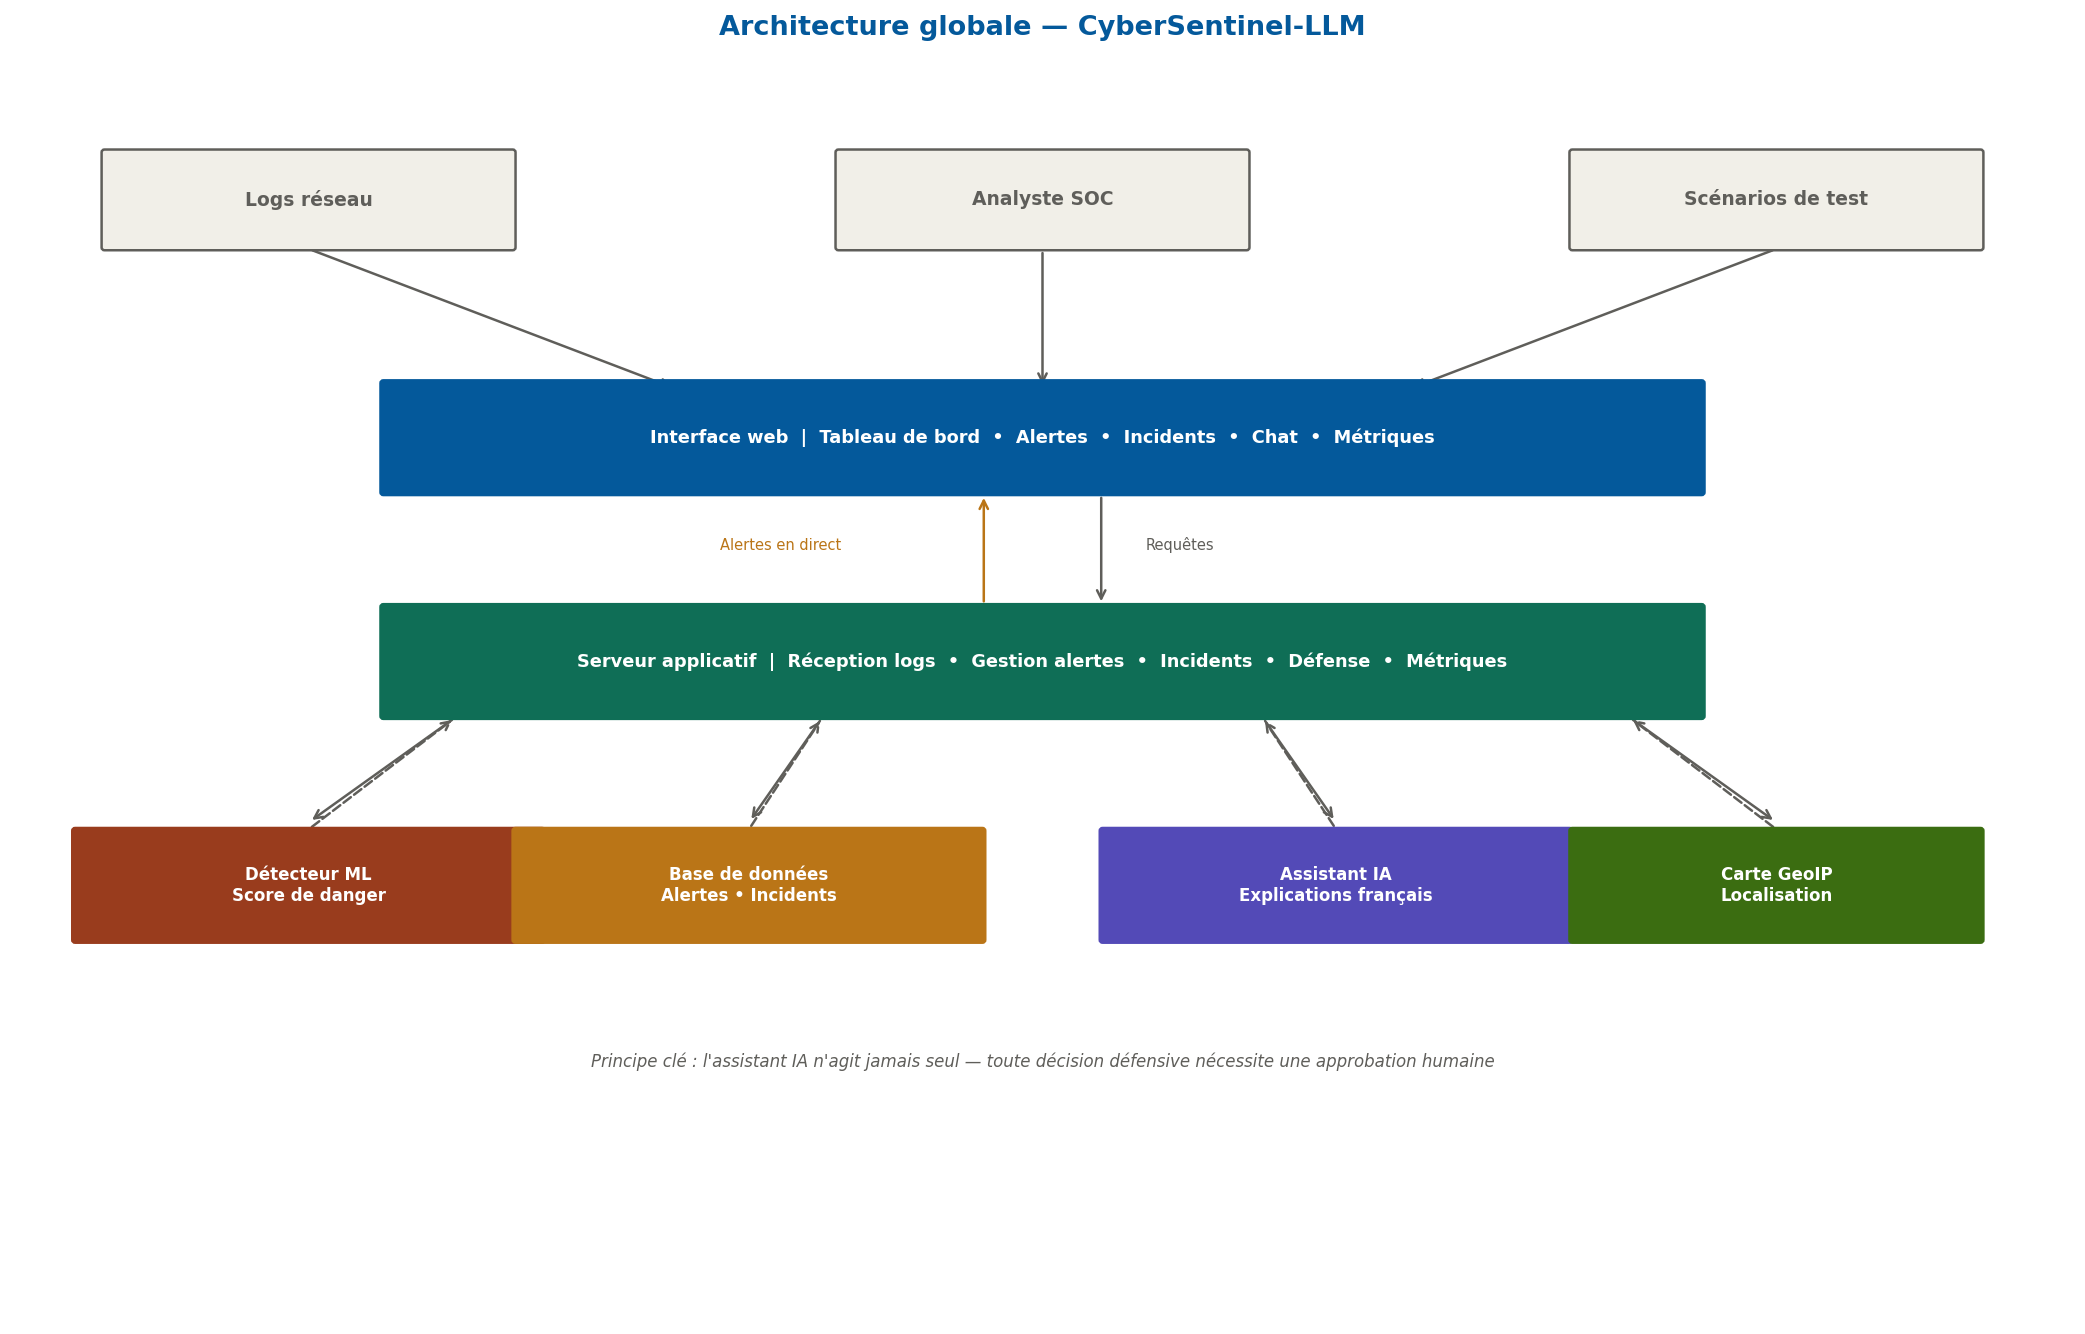
\includegraphics[width=0.90\linewidth]{images/cybersentinel_architecture.png}
\caption{Architecture globale de CyberSentinel-LLM}
\label{fig:annexe_architecture}
\end{figure}
\newpage

%% --- Annexe B ---
\section*{Annexe B : Exemples de payloads API}
\addcontentsline{toc}{section}{Annexe B : Exemples de payloads API}

\textbf{POST /ingest/logs — Requête et réponse :}

\begin{tcolorbox}[colback=lightblue, colframe=darkblue, arc=5pt]
\begin{small}
\begin{verbatim}
// Requête
{
  "ts": "2025-04-09T14:32:00Z",
  "source": "ssh",
  "ip": "185.220.101.45",
  "user": "root",
  "status": "fail"
}

// Réponse — Alerte créée
{
  "id": 42,
  "ts": "2025-04-09T14:32:00Z",
  "source": "ssh",
  "ip": "185.220.101.45",
  "rule": "ml_iforest_anomaly",
  "severity": "high",
  "score": 0.87,
  "status": "open"
}
\end{verbatim}
\end{small}
\end{tcolorbox}

\textbf{POST /defense/actions/\{id\}/approve — Réponse avec iptables :}

\begin{tcolorbox}[colback=lightblue, colframe=darkblue, arc=5pt]
\begin{small}
\begin{verbatim}
{
  "ok": true,
  "message": "IP 185.220.101.45 ajoutée à la liste noire applicative",
  "expires_at": "2025-04-09T15:02:00",
  "iptables_command": "iptables -A INPUT -s 185.220.101.45 -j DROP",
  "iptables_unblock": "iptables -D INPUT -s 185.220.101.45 -j DROP"
}
\end{verbatim}
\end{small}
\end{tcolorbox}
\newpage

%% --- Annexe C ---
\section*{Annexe C : Guide d'installation et d'exécution}
\addcontentsline{toc}{section}{Annexe C : Guide d'installation}

\textbf{Prérequis :}
\begin{itemize}
  \item[\ding{43}] Python 3.10+ avec pip
  \item[\ding{43}] Node.js 18+ avec npm
  \item[\ding{43}] Ollama installé avec le modèle qwen2.5:1.5b
  (\texttt{ollama pull qwen2.5:1.5b})
  \item[\ding{43}] GeoLite2-City.mmdb (optionnel, pour GeoIP)
\end{itemize}

\textbf{Lancement du backend :}
\begin{tcolorbox}[colback=lightblue, colframe=darkblue, arc=5pt]
\begin{small}
\begin{verbatim}
cd backend
pip install -r requirements.txt
uvicorn app.main:app --reload
# API disponible sur http://localhost:8000
# RAG initialisé automatiquement au démarrage
# Documentation Swagger : http://localhost:8000/docs
\end{verbatim}
\end{small}
\end{tcolorbox}

\textbf{Lancement du frontend :}
\begin{tcolorbox}[colback=lightblue, colframe=darkblue, arc=5pt]
\begin{small}
\begin{verbatim}
cd frontend
npm install
npm run dev
# Interface disponible sur http://localhost:3000
\end{verbatim}
\end{small}
\end{tcolorbox}

\begin{table}[!h]
\centering
\caption{Variables d'environnement principales}
\begin{tabular}{|p{5.5cm}|p{3cm}|p{5cm}|}
\hline
\textbf{Variable} & \textbf{Défaut} & \textbf{Description} \\
\hline
\texttt{OLLAMA\_BASE\_URL} & localhost:11434 & URL du serveur Ollama \\
\hline
\texttt{OLLAMA\_MODEL} & qwen2.5:1.5b & Modèle LLM utilisé \\
\hline
\texttt{SCORE\_THRESHOLD} & 0.6 & Seuil de détection ML \\
\hline
\texttt{DETECTOR} & hybrid & IF / LOF / hybrid \\
\hline
\texttt{DEFENSE\_MODE} & assist & off/monitor/assist/auto \\
\hline
\texttt{DEFENSE\_BLOCK\_TTL\_MINUTES} & 30 & Durée blocage temporaire \\
\hline
\texttt{DEFENSE\_ENFORCE\_API} & false & Active middleware HTTP 403 \\
\hline
\texttt{GEOLITE2\_CITY\_DB} & (optionnel) & Chemin base GeoIP \\
\hline
\texttt{APP\_ENV} & dev & dev ou production \\
\hline
\end{tabular}
\end{table}

\end{document}